\documentclass[bsc,logo,twoside,fullspacing,parskip]{infthesis}
%DIF LATEXDIFF DIFFERENCE FILE
%DIF DEL olddiss2.tex       Tue Mar 27 13:05:12 2018
%DIF ADD dissertation.tex   Tue Mar 27 13:04:28 2018
\usepackage{url}
\usepackage{graphicx}
\usepackage{appendix}
\usepackage{listings}
\usepackage{physics}
\usepackage{enumitem}
\usepackage{algorithm}
\usepackage{algorithmic}
\usepackage{array}
%DIF PREAMBLE EXTENSION ADDED BY LATEXDIFF
%DIF UNDERLINE PREAMBLE %DIF PREAMBLE
\RequirePackage[normalem]{ulem} %DIF PREAMBLE
\RequirePackage{color}\definecolor{RED}{rgb}{1,0,0}\definecolor{BLUE}{rgb}{0,0,1} %DIF PREAMBLE
\providecommand{\DIFadd}[1]{{\protect\color{blue}\uwave{#1}}} %DIF PREAMBLE
\providecommand{\DIFdel}[1]{{\protect\color{red}\sout{#1}}}                      %DIF PREAMBLE
%DIF SAFE PREAMBLE %DIF PREAMBLE
\providecommand{\DIFaddbegin}{} %DIF PREAMBLE
\providecommand{\DIFaddend}{} %DIF PREAMBLE
\providecommand{\DIFdelbegin}{} %DIF PREAMBLE
\providecommand{\DIFdelend}{} %DIF PREAMBLE
%DIF FLOATSAFE PREAMBLE %DIF PREAMBLE
\providecommand{\DIFaddFL}[1]{\DIFadd{#1}} %DIF PREAMBLE
\providecommand{\DIFdelFL}[1]{\DIFdel{#1}} %DIF PREAMBLE
\providecommand{\DIFaddbeginFL}{} %DIF PREAMBLE
\providecommand{\DIFaddendFL}{} %DIF PREAMBLE
\providecommand{\DIFdelbeginFL}{} %DIF PREAMBLE
\providecommand{\DIFdelendFL}{} %DIF PREAMBLE
\newcommand{\DIFscaledelfig}{0.5}
%DIF HIGHLIGHTGRAPHICS PREAMBLE %DIF PREAMBLE
\RequirePackage{settobox} %DIF PREAMBLE
\RequirePackage{letltxmacro} %DIF PREAMBLE
\newsavebox{\DIFdelgraphicsbox} %DIF PREAMBLE
\newlength{\DIFdelgraphicswidth} %DIF PREAMBLE
\newlength{\DIFdelgraphicsheight} %DIF PREAMBLE
% store original definition of \includegraphics %DIF PREAMBLE
\LetLtxMacro{\DIFOincludegraphics}{\includegraphics} %DIF PREAMBLE
\newcommand{\DIFaddincludegraphics}[2][]{{\color{blue}\fbox{\DIFOincludegraphics[#1]{#2}}}} %DIF PREAMBLE
\newcommand{\DIFdelincludegraphics}[2][]{% %DIF PREAMBLE
\sbox{\DIFdelgraphicsbox}{\DIFOincludegraphics[#1]{#2}}% %DIF PREAMBLE
\settoboxwidth{\DIFdelgraphicswidth}{\DIFdelgraphicsbox} %DIF PREAMBLE
\settoboxtotalheight{\DIFdelgraphicsheight}{\DIFdelgraphicsbox} %DIF PREAMBLE
\scalebox{\DIFscaledelfig}{% %DIF PREAMBLE
\parbox[b]{\DIFdelgraphicswidth}{\usebox{\DIFdelgraphicsbox}\\[-\baselineskip] \rule{\DIFdelgraphicswidth}{0em}}\llap{\resizebox{\DIFdelgraphicswidth}{\DIFdelgraphicsheight}{% %DIF PREAMBLE
\setlength{\unitlength}{\DIFdelgraphicswidth}% %DIF PREAMBLE
\begin{picture}(1,1)% %DIF PREAMBLE
\thicklines\linethickness{2pt} %DIF PREAMBLE
{\color[rgb]{1,0,0}\put(0,0){\framebox(1,1){}}}% %DIF PREAMBLE
{\color[rgb]{1,0,0}\put(0,0){\line( 1,1){1}}}% %DIF PREAMBLE
{\color[rgb]{1,0,0}\put(0,1){\line(1,-1){1}}}% %DIF PREAMBLE
\end{picture}% %DIF PREAMBLE
}\hspace*{3pt}}} %DIF PREAMBLE
} %DIF PREAMBLE
\LetLtxMacro{\DIFOaddbegin}{\DIFaddbegin} %DIF PREAMBLE
\LetLtxMacro{\DIFOaddend}{\DIFaddend} %DIF PREAMBLE
\LetLtxMacro{\DIFOdelbegin}{\DIFdelbegin} %DIF PREAMBLE
\LetLtxMacro{\DIFOdelend}{\DIFdelend} %DIF PREAMBLE
\DeclareRobustCommand{\DIFaddbegin}{\DIFOaddbegin \let\includegraphics\DIFaddincludegraphics} %DIF PREAMBLE
\DeclareRobustCommand{\DIFaddend}{\DIFOaddend \let\includegraphics\DIFOincludegraphics} %DIF PREAMBLE
\DeclareRobustCommand{\DIFdelbegin}{\DIFOdelbegin \let\includegraphics\DIFdelincludegraphics} %DIF PREAMBLE
\DeclareRobustCommand{\DIFdelend}{\DIFOaddend \let\includegraphics\DIFOincludegraphics} %DIF PREAMBLE
\LetLtxMacro{\DIFOaddbeginFL}{\DIFaddbeginFL} %DIF PREAMBLE
\LetLtxMacro{\DIFOaddendFL}{\DIFaddendFL} %DIF PREAMBLE
\LetLtxMacro{\DIFOdelbeginFL}{\DIFdelbeginFL} %DIF PREAMBLE
\LetLtxMacro{\DIFOdelendFL}{\DIFdelendFL} %DIF PREAMBLE
\DeclareRobustCommand{\DIFaddbeginFL}{\DIFOaddbeginFL \let\includegraphics\DIFaddincludegraphics} %DIF PREAMBLE
\DeclareRobustCommand{\DIFaddendFL}{\DIFOaddendFL \let\includegraphics\DIFOincludegraphics} %DIF PREAMBLE
\DeclareRobustCommand{\DIFdelbeginFL}{\DIFOdelbeginFL \let\includegraphics\DIFdelincludegraphics} %DIF PREAMBLE
\DeclareRobustCommand{\DIFdelendFL}{\DIFOaddendFL \let\includegraphics\DIFOincludegraphics} %DIF PREAMBLE
%DIF END PREAMBLE EXTENSION ADDED BY LATEXDIFF

\begin{document}

\title{Parallel Massive Dataset Cleaning}
\author{Jianmeng Yu}
\course{Computer Science}
\project{4th Year Project Report}
\date{\today}

\DIFdelbegin %DIFDELCMD < \abstract{
%DIFDELCMD < \pagenumbering{roman}
%DIFDELCMD < This project applies the decision algorithm\cite{Pugh} developed by Pugh on a massive parallel scale. This aims to remove a large amount of False Positive fish detections in the Fish4Knowledge (F4K) dataset\cite{F4K}, without losing too many True Positives.
%DIFDELCMD < 

%DIFDELCMD < According to Qiqi Yu's estimated runtime\cite{Yu}, the cleaning process will take more than 1000 days to complete on a 40-core machine. Simply running the process on a parallel scale will not be sufficient, optimization of the code is also essential for making the processing more feasible.
%DIFDELCMD < 

%DIFDELCMD < This document describes the detail of various approach to reduce unnecessary work during pre-processing and improve the cleaning algorithm. In this process, efficiency evaluation for different implementations of the machine learning techniques is used to reduce computational time cost. 
%DIFDELCMD < A more detailed roadmap this project is provided in Chapter 1.
%DIFDELCMD < 

%DIFDELCMD < }
%DIFDELCMD < %%%
\DIFdelend \DIFaddbegin \abstract{
\pagenumbering{roman}
This project adopts the decision algorithm\cite{Pugh} developed by Pugh on a massive parallel scale. This aims to remove a large amount of False Positive fish detections in the Fish4Knowledge (F4K) dataset\cite{F4K}, without losing too many True Positives.

According to Qiqi Yu's estimated runtime\cite{Yu}, the cleaning process will take more than 1000 days to complete on a 40-core machine. Simply running the process on a parallel scale will not be sufficient, optimization of the code is also essential for making the processing more feasible.

This document describes the detail of various approaches to reduce unnecessary work during pre-processing and improve the cleaning algorithm. In this process, evaluation of efficiency for different implementations of machine learning techniques is used to reduce computational time cost. 

After translating and optimizing the decision algorithm, the project distributed the task to 200 4-core machines and finishes the decision algorithm in 10 days.
However, due to a mistake in previous work the cleaning does not achieve the expected accuracy, only 42\% of the bad detections were removed instead of 90\%, at the lost of 7\% of good fishes. 
The cleaning process reduces the total data size by 27.8\%, which saves about 600 GB of disk space.

A more detailed roadmap this project is provided in Chapter 1.



}
\DIFaddend 

\maketitle

\section*{Acknowledgements}
I would like to thank my project supervisor, Prof. Fisher, for his constant, patient support throughout the year. Without his expert knowledge in the field, it would be impossible for me to navigate through all of the data source and prior work of the Fish4Knowledge project. 

I would also like to thank Mr \DIFdelbegin \DIFdel{. }\DIFdelend Matthew Pugh for spending time answering my questions on the project \DIFdelbegin \DIFdel{, }\DIFdelend and precious advice on the implementation of his algorithms.

I must also extend gratitude to my friends, and my family back in China, for all their help and encouragement during my study.

\newpage

\standarddeclaration

\tableofcontents



\chapter{Introduction}

\pagenumbering{arabic}

The main goal of this project is to produce a cleaned subset of a 1.6 TB dataset for future research purposes. And the main challenge of the project is to re-engineer the framework used to make it more scalable, hence finish the 800,000-hour task within a reasonable amount of time.

\section{Fish4Knowledge Project (F4K)}

The Fish4Knowledge (F4K) project, funded by EU's Seventh Framework Programme (FP7), studied \DIFdelbegin \DIFdel{environmental effects }\DIFdelend \DIFaddbegin \DIFadd{ecological issues }\DIFaddend by analysing raw videos and extracting information from it, so researchers could use \DIFdelbegin \DIFdel{it }\DIFdelend \DIFaddbegin \DIFadd{the data }\DIFaddend for studies without much programming skills. 

The project acquired video data collected by Taiwan Ocean Research Institute. 
They set up 9 cameras in different coral reef areas in Taiwan such as Nanwan National Park (NPP-3), Lanyu, and Houbi Lake (HoBiHu). 
The project collected 5 years of recording, about 524,000 10-minute video clips with a total size of 91 TB. Approximately 1.4 billion fish \DIFdelbegin \DIFdel{detection }\DIFdelend \DIFaddbegin \DIFadd{detections }\DIFaddend found in the videos\DIFdelbegin \DIFdel{, we }\DIFdelend \DIFaddbegin \DIFadd{. 
We }\DIFaddend call this the F4K Original Data Set (FDS). 

Attempting to reduce the dataset, the F4K project developed and applied a species recognition algorithm. 
This algorithm extracts all detections as 100x100 RGB images and their description files, reducing the dataset to approximately 839 million detections, having a combined size of 1.6 TB
This dataset is called Reduced FDS (RDS)\DIFdelbegin \DIFdel{, a }\DIFdelend \DIFaddbegin \DIFadd{.
A }\DIFaddend more detailed composition of these files \DIFdelbegin \DIFdel{are }\DIFdelend \DIFaddbegin \DIFadd{is }\DIFaddend described in Chapter \ref{chap:datasource}.

\section{Project Motivation}

In 2015, Pugh\cite{Pugh} developed a cleaning algorithm for RDS based on Huang's thesis\cite{Huang}, which would approximately remove 90\% of the False Positives (objects that are not fish, recognized as fish), while only losing about 8\% of True Positives (true fish detections). 

However, due to lack of time and resource, the framework is not implemented and the cleaning was not applied \DIFdelbegin \DIFdel{on }\DIFdelend \DIFaddbegin \DIFadd{to }\DIFaddend the full dataset.
In 2016, Yu\cite{Yu} \DIFdelbegin \DIFdel{attempted to add }\DIFdelend \DIFaddbegin \DIFadd{added }\DIFaddend voting constraints on the cleaning algorithm, to both increase accuracy and reduce runtime\DIFdelbegin \DIFdel{, after evaluation}\DIFdelend \DIFaddbegin \DIFadd{. 
After evaluation, }\DIFaddend it's estimated this constraint \DIFdelbegin \DIFdel{could }\DIFdelend \DIFaddbegin \DIFadd{did }\DIFaddend reduce the time cost of the algorithm for about 10\%, at cost of 5\% of accuracy.

Even after the reduction by Yu, it's evaluated the cleaning algorithm would still \DIFdelbegin \DIFdel{took }\DIFdelend \DIFaddbegin \DIFadd{take }\DIFaddend 25,000 hours on a 40-core machine\cite{Yu}.
This means simply put the task on parallel would not be sufficient, distributed computing over more machines is needed.
For this purpose, the project uses the lab machines provided by the University of Edinburgh for cleaning. 
Even with about 800 cores available, the algorithm would still \DIFdelbegin \DIFdel{took }\DIFdelend \DIFaddbegin \DIFadd{take }\DIFaddend more than 1,000 \DIFdelbegin \DIFdel{hour }\DIFdelend \DIFaddbegin \DIFadd{hours }\DIFaddend to finish, this the code should be also optimized for the project to be more scalable.

\section{Project Outcome}

The project manages to reduce the total runtime by 50\% after translating the pipeline classifier developed by Pugh\cite{Pugh}, and removing unnecessary operations in it. 
It is predicted that this classifier reduces the dataset by about 28\%, with the following statistics:
\newcolumntype{C}{>$c<$}
\DIFdelbegin %DIFDELCMD < \newcolumntype{C}{>$c<$}
%DIFDELCMD < %%%
\[
\DIFdel{\begin{array}{C|C|C}
$ $ & Predicted Fish & Predicted Non-Fish \\
\hline 
True Fish & 92.528\% & 7.472\% \\
Non Fish & 57.980\% & 42.020\%
\end{array}
}\]
%DIFAUXCMD
\DIFdelend \DIFaddbegin \begin{center}
\begin{tabular}{ |c|c|c| }
\hline 
\DIFadd{$ $ }& \DIFadd{Predicted Fish }& \DIFadd{Predicted Non-Fish }\\
\hline 
\DIFadd{True Fish }& \DIFadd{92.528\% }& \DIFadd{7.472\% }\\
\DIFadd{Non Fish }& \DIFadd{57.980\% }& \DIFadd{42.020\% }\\
\hline 
\end{tabular}
\end{center}
\DIFaddend 

However\DIFaddbegin \DIFadd{, }\DIFaddend this does not meet the expectation from Pugh's thesis, whereas 90\% of the False Positive is removed. 
This is caused by \DIFdelbegin \DIFdel{a }\DIFdelend \DIFaddbegin \DIFadd{an }\DIFaddend extraction mistake in preprocessing stage, which causes the CNN trained becoming useless. 
Re-training the CNN could increase the accuracy, but it is not used due to \DIFaddbegin \DIFadd{the }\DIFaddend limit of time and resource.

%DIF < more machines is needed to change the scope into distributed parallel processing, 
%DIF < The cleaning wasn't applied because the constraint could not improve much to the efficiency of cleaning.
\DIFdelbegin %DIFDELCMD < 

%DIFDELCMD < %%%
%DIF < It is evaluated cleaning a 1,000 detection video on a 40-core machine would take 200 seconds.
%DIF < This gives a 8 second per frame per core (8 {\tt s/fc}), with the available 200 4-core machines in student labs, 1 {\tt s/fc} would result in 12 days of computational time.
%DIFDELCMD < 

%DIFDELCMD < %%%
\DIFdelend \section{Contribution}

During this project, the parallel task distribution programme is based on a public GitHub repository \DIFdelbegin \DIFdel{"}\DIFdelend \DIFaddbegin \DIFadd{``}\DIFaddend mpi-master-slave\DIFdelbegin \DIFdel{" }\DIFdelend \DIFaddbegin \DIFadd{'' }\DIFaddend created by user \DIFdelbegin \DIFdel{"}\DIFdelend \DIFaddbegin \DIFadd{``}\DIFaddend luca-s\DIFdelbegin \DIFdel{"\mbox{%DIFAUXCMD
\cite{L5}}%DIFAUXCMD
, minor }\DIFdelend \DIFaddbegin \DIFadd{''\mbox{%DIFAUXCMD
\cite{L5}}%DIFAUXCMD
, some }\DIFaddend changes were made to the work queue and protocol for thrashing prevention and crash recovery, the pseudo-code of this framework is provided in Appendix \ref{apped:msf}.

\DIFdelbegin \DIFdel{Data extraction pipeline written in Python was created }\DIFdelend \DIFaddbegin \DIFadd{A data extraction pipeline was created in Python }\DIFaddend to partition, extract, and parse the raw SQL dump file to \DIFdelbegin \DIFdel{comma separated values }\DIFdelend \DIFaddbegin \DIFadd{Comma Separated Values }\DIFaddend stored in plain text files, this removes the need of maintaining a SQL server and speeds up the extraction. 

The pipeline classifier is also re-written in Python, \DIFaddbegin \DIFadd{and the }\DIFaddend unfinished part of the original pipeline is implemented. 
Due to the removal of the SQL server in the pipeline, the extraction and visualization MATLAB scripts created by Pugh are re-written into Python functions. 
Some \DIFdelbegin \DIFdel{metrics algorithms used is }\DIFdelend \DIFaddbegin \DIFadd{metric algorithms were }\DIFaddend translated from MATLAB for loops to Numpy/Scipy operations to increase efficiency.

F4K project's feature extraction MATLAB code developed by Huang\cite{Huang} is \DIFdelbegin \DIFdel{untranslated }\DIFdelend \DIFaddbegin \DIFadd{not translated }\DIFaddend and is called within Python using PyMatlab library. Some minor changes like replacing \DIFaddbegin \DIFadd{the }\DIFaddend edge extraction algorithm used \DIFdelbegin \DIFdel{, }\DIFdelend and error handling \DIFaddbegin \DIFadd{were }\DIFaddend added to some of the unstable functions. 

For validation of Pugh's classifier performance, a separate set of videos were \DIFdelbegin \DIFdel{marked}\DIFdelend \DIFaddbegin \DIFadd{ground-truthed}\DIFaddend . After testing the classifiers on this dataset, it's discovered that Pugh's classifiers over-fits on the training dataset. Also by inspecting the training code, it is found that the training set \DIFdelbegin \DIFdel{were }\DIFdelend \DIFaddbegin \DIFadd{was }\DIFaddend heavily biased. A new complementary ground truth dataset \DIFdelbegin \DIFdel{were marked }\DIFdelend \DIFaddbegin \DIFadd{was created }\DIFaddend for training new classifiers. 

The classification step was originally going to use Pugh's trained SVM and CNN. Due to the problem above, the SVM parameters used are re-calibrated for higher accuracy on \DIFaddbegin \DIFadd{the }\DIFaddend unseen dataset. 
The Python's {\tt sklearn.svm.SVC} \DIFdelbegin \DIFdel{were }\DIFdelend \DIFaddbegin \DIFadd{was }\DIFaddend used to achieve the same result instead of translation. The CNN implemented with \DIFdelbegin \DIFdel{lua }\DIFdelend \DIFaddbegin \DIFadd{Lua }\DIFaddend torch are rewritten and called with Lutorpy library.
A fatal mistake \DIFdelbegin \DIFdel{were }\DIFdelend \DIFaddbegin \DIFadd{was }\DIFaddend found in the CNN design, after evaluating the result with voting strategy, it is discovered the CNN trained \DIFdelbegin \DIFdel{by Pugh }\DIFdelend were almost useless. Details about the fault and the \DIFdelbegin \DIFdel{re-train attempt }\DIFdelend \DIFaddbegin \DIFadd{re-training attempts }\DIFaddend were included in Section \ref{sec:cnn}.

Reconstruction of the videos \DIFdelbegin \DIFdel{were }\DIFdelend \DIFaddbegin \DIFadd{was }\DIFaddend not applied due to the low accuracy, a binary decision vector \DIFdelbegin \DIFdel{were }\DIFdelend \DIFaddbegin \DIFadd{was }\DIFaddend generated instead.

\section{Document Structure}

\textbf{Chapter \ref{chap:bg}} discusses the previous work and designs details used in the project. 

\textbf{Chapter \ref{chap:datasource}} described the details of the data sources, storage and preprocessing used in the cleaning algorithm.

\textbf{Chapter \ref{chap:prepro}} describes the first stages of the cleaning: early detection removal, feature extraction, preprocessing for classification in the next stage.

\textbf{Chapter \ref{chap:classify}} discusses the final classifiers used in the cleaning, with evaluation of the results and comparison between different algorithms. 

%\textbf{Chapter \ref{chap:voting}} described the voting strategies to increase the accuracy of classifiers.

\textbf{Chapter \ref{chap:parallel}} talks about the task distribution system used in this project \DIFdelbegin \DIFdel{, }\DIFdelend and some of the difficulties and solutions.

\textbf{Chapter \ref{chap:conclusion}} contains the conclusions and possible future work needed for the project.
\newpage


\chapter{\DIFdelbegin \DIFdel{Backgrounds}\DIFdelend \DIFaddbegin \DIFadd{Background}\DIFaddend }
\label{chap:bg}

\section{Big Data and Distributed Computing}

Big data is one of the hottest trending topics recently, where the amount of the data generated is not possible to be manually analysed. 
Different to the popular text stream \DIFdelbegin \DIFdel{analysing, the }\DIFdelend \DIFaddbegin \DIFadd{analysis, this }\DIFaddend project is more focused on image processing of a large collection. 
There are already some image processing libraries with work distribution framework\DIFdelbegin \DIFdel{, for }\DIFdelend \DIFaddbegin \DIFadd{. For }\DIFaddend example: Hadoop Image Processing Interface\cite{L3}, \DIFaddbegin \DIFadd{an }\DIFaddend Apache Spark based 4Quant\cite{L4} \DIFdelbegin \DIFdel{, }\DIFdelend and other tool-kits for distributed parallelization.

Due to the limit of the project scale, the project could not use dedicated servers for cleaning the dataset.
Instead, this project \DIFdelbegin \DIFdel{uses }\DIFdelend \DIFaddbegin \DIFadd{used }\DIFaddend the student lab machines provided by The University of Edinburgh.
These machines have \DIFaddbegin \DIFadd{the }\DIFaddend Distributed Informatics Computing Environment (DICE) desktop installed, and using Andrew File System (AFS) for storage, this provides immense convenience on the project's need of fast and distributed I/O.
Approximately 200-300 student lab DICE \DIFaddbegin \DIFadd{machines}\DIFaddend , a 1 TB and 256 GB disk space on AFS were used for this project.

The DICE machines used in the project \DIFdelbegin \DIFdel{does }\DIFdelend \DIFaddbegin \DIFadd{do }\DIFaddend not have a shared memory\DIFdelbegin \DIFdel{, this }\DIFdelend \DIFaddbegin \DIFadd{. 
This }\DIFaddend means the project will also need tools for distribution of the task before \DIFaddbegin \DIFadd{being }\DIFaddend parallelized locally.
Since a shared file system is already provided, the more standard and portable Message Passing Interface (MPI) is used for distribution of the task. 
More specifically, the MPI4PY\cite{MPI4PY}, \DIFdelbegin \DIFdel{a }\DIFdelend \DIFaddbegin \DIFadd{an }\DIFaddend MPI library designed for Python is used for this project\DIFdelbegin \DIFdel{, details }\DIFdelend \DIFaddbegin \DIFadd{. Details }\DIFaddend of the task distribution design used are described in Chapter \ref{chap:parallel}.

\section{Classification Schema}
\label{sec:schema}

The reduction procedure of F4K project removed some of the False Positives from FDS. 
However, there are still a lot of False Positives in the RDS\DIFdelbegin \DIFdel{, to }\DIFdelend \DIFaddbegin \DIFadd{. 
To }\DIFaddend resolve this issue, a classification schema is created to identify the detections.

In \DIFaddbegin \DIFadd{the }\DIFaddend previous work of Pugh\cite{Pugh}, ten different detection classes were used to ground truth the dataset, which is later used to train different classifiers used in the cleaning. 

These 10 classes can be divided into 3 main categories (with examples in Fig \ref{fig:classes}):

\renewcommand{\labelenumi}{\bfseries\Roman{enumi}}
\renewcommand{\labelenumii}{\bfseries\arabic{enumii}}
\renewcommand{\labelenumiii}{\bfseries\roman{enumiii}}

\begin{enumerate}
   \setlength{\parskip}{3pt}

 \item \textbf{Not A Fish} - These \DIFdelbegin \DIFdel{detection }\DIFdelend \DIFaddbegin \DIFadd{detections }\DIFaddend are marked for removal in future.
 \begin{enumerate}
   \item \textbf{Compression Artefact} - During the process of recording video, some bits were dropped during transmission of the compressed video. These detections usually have rigid square shapes.
   \item \textbf{Illumination Artefact} - Changes of brightness recognized as fish, they are usually refraction caused by turbid water, or light reflecting plankton.
   \item \textbf{Background Vegetation} - Some of the \DIFdelbegin \DIFdel{video }\DIFdelend \DIFaddbegin \DIFadd{videos }\DIFaddend are captured with dynamic backgrounds, where the swaying plants are recognized as fish.
   \item \textbf{Others} - Everything else, this includes large floating matter, empty contours created by faults in previous algorithms.
   \item \textbf{Unknown} - Due to issues like lighting, blurry and stretched video frames, it's uncertain the detection is fish or not.
 \end{enumerate}

 \item \textbf{A Fish} - These frames are useful for future researchers.
 \begin{enumerate}
   \setcounter{enumii}{5} 
   \item \textbf{Good Boundary} - With clear ocean as background, these fish have good boundaries, and are useful for future species recognition.
   \item \textbf{Partial Fish} - Mostly good detection boundary, but part of the fish is cut-off for various reasons:
    \begin{enumerate}
      \item Fishes cut by frame boundaries.
      \item Fishes are covered by vegetation or other fishes.
      \item The fish is too big and cropped by the 100x100 boundary.
    \end{enumerate}
   \item \textbf{Bad Boundary} - The fish is clearly captured, but the boundary extracted is erratic and useless for research. 
 \end{enumerate}

 \item \textbf{A Fish, but not useful} - These frames \DIFdelbegin \DIFdel{detects fishcorrectly}\DIFdelend \DIFaddbegin \DIFadd{detections are true fish}\DIFaddend , but misleading information may be extracted\DIFdelbegin \DIFdel{, it}\DIFdelend \DIFaddbegin \DIFadd{. It}\DIFaddend 's unsure these frames should be kept or not.
 \begin{enumerate}
   \setcounter{enumii}{8} 
   \item \textbf{Other Errors} - like compression artefact are found in the image.
   \item \textbf{Multiple Fish} - with shared contour.
 \end{enumerate}
\end{enumerate}

However, this classification schema was not good enough for evaluating \DIFaddbegin \DIFadd{the }\DIFaddend accuracy of the classifiers due to the similarity between the classes, this limitation and the possible improvements are described in Section \ref{sec:AmbigCS}.

\begin{figure}
    \centering
    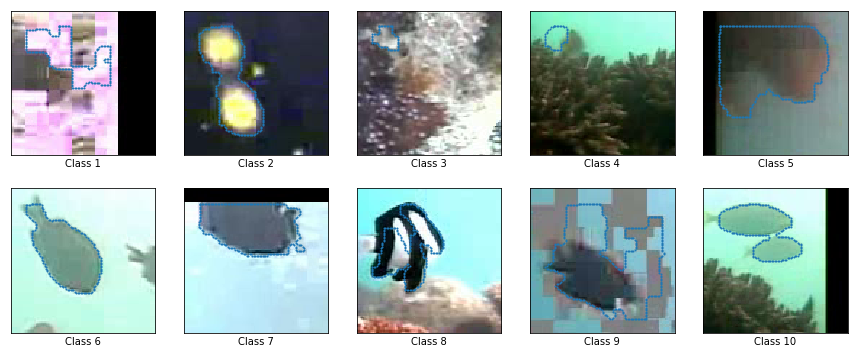
\includegraphics[scale=0.4]{graph/class_sample.png}
    \caption{Example Detections From Each Class}
    \label{fig:classes}
\end{figure}

\section{Pipeline Classifier}

The main part of the project is to translate and apply the pipeline classifier, designed by Pugh\cite{Pugh}. 
However, under limitations, the pipeline itself could not be applied directly on a parallel scale in this project.

The first limitation is the SQL database, which stores the track and contour information of the image. 
However\DIFaddbegin \DIFadd{, }\DIFaddend the SQL database is too large and is estimated to be slow for the project.
To make the extraction more sensible, a Python script was used to partition the raw {\tt .SQL} file, this removed the need for a SQL database server. 
More details of this modification \DIFdelbegin \DIFdel{is }\DIFdelend \DIFaddbegin \DIFadd{are }\DIFaddend in Section \ref{sec:sqld}.

%The data pre-processing is the slowest part of the pipeline after removing the SQL server. 
In Pugh's thesis\cite{Pugh}, a Frame Edge Indicator Function (FEIF) is used to directly reduce the number of frames \DIFaddbegin \DIFadd{that }\DIFaddend need to be classified\DIFdelbegin \DIFdel{, after }\DIFdelend \DIFaddbegin \DIFadd{. 
After }\DIFaddend improvements and some new additions on dataset reduction, pre-processing cleans out about 20\% of the detections. More details on the reduction are in Chapter \ref{chap:datasource}.

Before sending the data into the classifiers, preprocessing is needed to give a more sensible result.
The project uses feature extraction code from both Huang's\cite{Huang} and Pugh's\cite{Pugh} work, normalizing and transforming them with \DIFdelbegin \DIFdel{Pricipal }\DIFdelend \DIFaddbegin \DIFadd{Principal }\DIFaddend Component Analysis (PCA).
After extracting and reducing the features, they are fed into 3 Convolutional Neural Networks (CNN) and 10-class Support Vector Machine (SVM) to obtain the predicted probability of each class from each classifier.
Where a voting strategy \DIFdelbegin \DIFdel{were }\DIFdelend \DIFaddbegin \DIFadd{was }\DIFaddend used to combine the results from the classifiers into the final decision array.

Fig \ref{fig:pipeline} shows the steps used in the original pipeline classifier designed by Pugh.
Note that in this project, the SVM \DIFdelbegin \DIFdel{were }\DIFdelend \DIFaddbegin \DIFadd{was }\DIFaddend changed to a single \DIFdelbegin \DIFdel{multi-class SVM and top-N decision were }\DIFdelend \DIFaddbegin \DIFadd{Multi-class SVM and the Top-N Decision was }\DIFaddend replaced by a voting strategy.
\DIFaddbegin \DIFadd{See Chapter \ref{chap:classify} for more details.
}\DIFaddend 

\begin{figure}[!h]
    \centering
    \DIFdelbeginFL %DIFDELCMD < 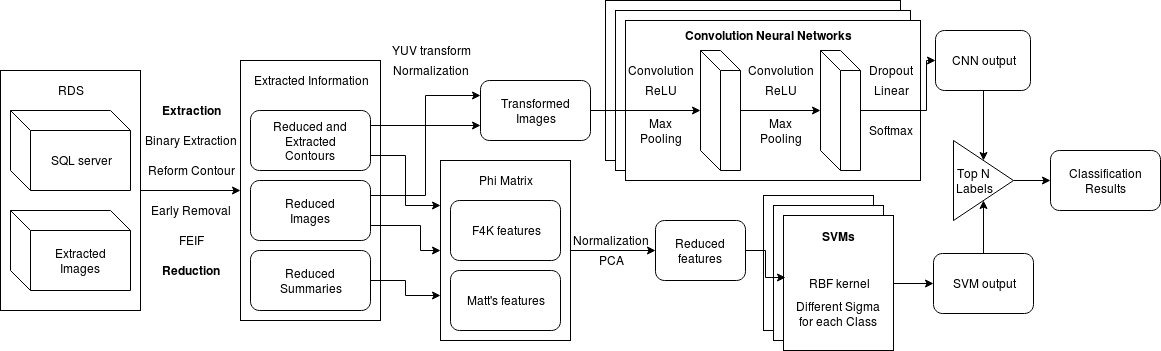
\includegraphics[scale=0.3]{graph/Pipeline_Classifier.png}
%DIFDELCMD <     %%%
\DIFdelendFL \DIFaddbeginFL 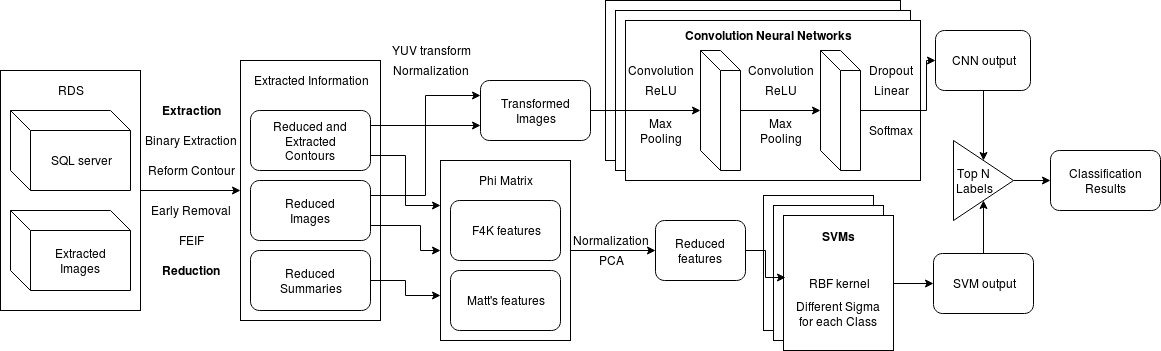
\includegraphics[scale=0.35]{graph/Pipeline_Classifier.png}
    \DIFaddendFL \caption{Pipeline Classifier designed by Pugh, modified}
    \label{fig:pipeline}
\end{figure}

\section{Yu's Voting Constraints}

In 2016, Yu\cite{Yu} tried to add a voting constraint \DIFdelbegin \DIFdel{on }\DIFdelend \DIFaddbegin \DIFadd{to }\DIFaddend the Pipeline Classifier. 
Yu evaluated her 3 voting \DIFdelbegin \DIFdel{method on the result }\DIFdelend \DIFaddbegin \DIFadd{methods on the results }\DIFaddend obtained by Pugh \DIFdelbegin \DIFdel{, }\DIFdelend and tested it against the obtained result of the Top-N method. 
Yu's evaluation discovered that this method would reduce the total runtime by 10\%\DIFdelbegin \DIFdel{, however this process decrease }\DIFdelend \DIFaddbegin \DIFadd{. 
However, this process decreases }\DIFaddend the True Positive Rate (TPR) by 5\% and is not considered useful for the project. 

\DIFdelbegin \DIFdel{However after }\DIFdelend \DIFaddbegin \DIFadd{After }\DIFaddend further evaluation of both Pugh and Yu's work, it is discovered that Pugh's final classifier over-fits on the training dataset due to \DIFdelbegin \DIFdel{the }\DIFdelend \DIFaddbegin \DIFadd{deep net }\DIFaddend coverage, and mistakes in preprocessing steps. Details of this problem \DIFdelbegin \DIFdel{is }\DIFdelend \DIFaddbegin \DIFadd{are }\DIFaddend discussed in Section \ref{sec:gt} and Section \ref{sec:CNNprepro}. 

\DIFdelbegin \DIFdel{Since Yu's evaluation were based on the results of Pugh's experimental classifiers, it is shown that Pugh's classifier would obtain promising accuracy if the mistake in Section \ref{sec:cnn} is fixed. 
Due to the high cost of training, this project tested a modified version of Qiqi's voting strategy to make use of the results from the over-fitted classifiers.
}\DIFdelend \DIFaddbegin \DIFadd{To fully utilise the results from the over-fitted classifiers, a voting approach similar to Yu's work was tested and applied. 
The final result will be obtained by voting of 4 classifiers, instead of using the Top-N function.
Detail of the voting strategy is included in Chapter \ref{sec:voting}.
}

%DIF > Due to the high cost of training, this project tested a modified version of Yu's voting strategy to make use of the results from the over-fitted classifiers. 
\DIFaddend %Detail of the modification and evaluation are included in Chapter \ref{sec:voting}.

\chapter{Data Source}
\label{chap:datasource}

The species recognition of the F4K project provided three types of output files:
\begin{itemize}
\setlength{\parskip}{1pt}
\item
Extracted 100x100 RGB images, compiled into {\tt .avi} video file.
\item
Corresponding summary of the video, recording detection id and bounding box sizes. Stored in \DIFdelbegin \DIFdel{comma separated values }\DIFdelend \DIFaddbegin \DIFadd{Comma Separated Values }\DIFaddend format, as {\tt .txt} file.
\item
A {\tt .sql} dump file of 500GB, from the database used for species extraction.
\end{itemize}

In the species recognition process, a {\tt video\_id} is generated for \DIFdelbegin \DIFdel{each video,}\DIFdelend \DIFaddbegin \DIFadd{every 400,000 videos, }\DIFaddend this consists of a 32 byte hash of video, a {\tt \#}, and the filming date in {\tt YYYYMMDDhhmm} format. \DIFdelbegin \DIFdel{Were }\DIFdelend \DIFaddbegin \DIFadd{Where }\DIFaddend each of the {\tt video\_id} have a corresponding {\tt .avi} and {\tt .txt} file.

\section{Extracted Images}
\label{sec:summaries}

The species recognition in F4K project extracted every detection with {\tt w} and {\tt h} both smaller than 90. 
This process is illustrated in Figure \ref{fig:extraction}, where a 100x100 area is selected with top left corner \DIFdelbegin \DIFdel{coordinate }\DIFdelend \DIFaddbegin \DIFadd{coordinates }\DIFaddend {\tt (w-10)} and {\tt (h-10)} and cropped from the image.
If the some of \DIFdelbegin \DIFdel{selected area are }\DIFdelend \DIFaddbegin \DIFadd{the selected areas is }\DIFaddend out of the frame, it will be filled with black pixels.

During this process, the contour and the bounding box of the fish were also calculated.
The bounding box consists of 4 values {\tt x,y,w,h}, where {\tt x} and {\tt y} are the coordinate of the top left corner, {\tt w} and {\tt h} are the width and height of the bounding box. 
Those cropped images are then stored in file {\tt summary\_(video\_id).avi}, with detection id and {\tt w} and {\tt h} stored in corresponding {\tt frame\_info\_(video\_id).txt}.

There are a total of 396,901 of such videos, consist of 839,465,846 frames, \DIFdelbegin \DIFdel{sums up to }\DIFdelend \DIFaddbegin \DIFadd{with }\DIFaddend a total size of 1.14 TB.

\begin{figure}
    \centering
    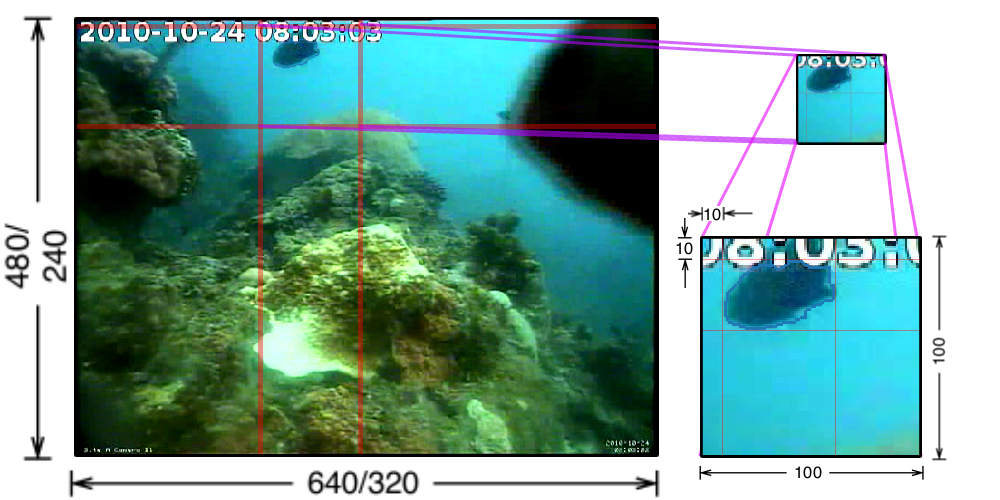
\includegraphics[scale=0.3]{graph/extraction.png}
    \caption{Process of Extracting Image}
    \label{fig:extraction}
\end{figure}

\section{SQL dump file}
\label{sec:sqld}

The {\tt .sql} dump file comes from the SQL workflow used in the F4K project, which means not the only details of fish detection are stored, other irrelevant components like user logs are also stored inside. 

In this project, only the \DIFdelbegin \DIFdel{"Fish Detection" and "Camera" table are }\DIFdelend \DIFaddbegin \DIFadd{``Fish Detection'' and ``Camera'' table is }\DIFaddend needed for the cleaning, hence extraction of the relevant information might be needed before the cleaning.
\DIFdelbegin \DIFdel{Below }\DIFdelend \DIFaddbegin \DIFadd{For example, below }\DIFaddend is the schema of the \DIFdelbegin \DIFdel{"Fish Detection" }\DIFdelend \DIFaddbegin \DIFadd{``Fish Detection'' }\DIFaddend table. 

\lstdefinestyle{sql}{
  language=SQL,
  tabsize=1,
  showspaces=false,
  showstringspaces=false
}
\lstset{basicstyle=\tiny\ttfamily,breaklines=true,style=sql}
\begin{lstlisting}[frame=single]
CREATE TABLE IF NOT EXISTS ‘f4k_db‘.‘fish_detection‘ (
‘detection_id‘ INT(11) NOT NULL AUTO_INCREMENT,
‘fish_id‘ INT(11) NOT NULL,
‘video_id‘ CHAR(45) CHARACTER SET ’utf8’ NOT NULL DEFAULT ’’,
‘frame_id‘ MEDIUMINT(9) NOT NULL DEFAULT ’0’,
‘timestamp‘ TIMESTAMP NOT NULL DEFAULT CURRENT_TIMESTAMP ON UPDATE CURRENT_TIMESTAMP,
‘bb_cc‘ BLOB NOT NULL,
‘detection_certainty‘ FLOAT NULL DEFAULT NULL,
‘tracking_certainty‘ FLOAT NULL DEFAULT NULL,
‘component_id‘ SMALLINT(6) NOT NULL,
‘processed_videos_id‘ INT(11) NOT NULL
\end{lstlisting}

This {\tt .sql} dump file is stored as plain text files that could be loaded with a SQL server.
Under limitations of disk space and access speed, loading such large SQL database dump file into a server and performing 400,000 queries is unnecessary and very time-consuming, hence making it the slowest part of the cleaning. 
A Python script with standard stream pipeline is used to parse and partition the SQL dump file into directly usable files instead.

\subsection{Standard Stream \DIFdelbegin \DIFdel{based }\DIFdelend \DIFaddbegin \DIFadd{Based }\DIFaddend Extraction Script}

In this project, each record needed for the cleaning is independent (given they have different video\_id). 
If each detection is stored in a corresponding \DIFdelbegin \DIFdel{files }\DIFdelend \DIFaddbegin \DIFadd{file }\DIFaddend with its video\_id, the information extraction will be much faster without the need to seek through all the records of other videos.

The project uses \DIFaddbegin \DIFadd{a }\DIFaddend standard stream pipeline because each detection is only \DIFdelbegin \DIFdel{need }\DIFdelend \DIFaddbegin \DIFadd{needed }\DIFaddend once during the extraction, and the dump file is too large to be loaded into the RAM.

With simple Python functions such as {\tt split()}, the \DIFdelbegin \DIFdel{record }\DIFdelend \DIFaddbegin \DIFadd{records }\DIFaddend in the dump file of form:
\lstset{basicstyle=\small\ttfamily,breaklines=true,style=sql}
\begin{lstlisting}[frame=single]
 INSERT INTO `fish_detection` VALUES (1),(2),(3),(4)...(N)
\end{lstlisting}
are parsed into directly usable \DIFdelbegin \DIFdel{list }\DIFdelend \DIFaddbegin \DIFadd{lists }\DIFaddend of values, separated by \DIFaddbegin \DIFadd{a }\DIFaddend {\tt newline} character.

Which reduces the time cost for loading the dataset reduced to an almost negligible amount. 
The output of this script contains 326 GB of {\tt .csv} files, each one corresponds to the associated {\tt video\_id}.

%In Qiqi's estimate, the loading and preprocessing would take 800,000 hours (25,000 hours on a 32 core machine) in the original design (double the time if considering her calculation error). After the pre-extraction, it only took about 0.3 seconds on average for a frame to be load and processed on a single computational thread. Which is about 70,000 hours, essentially cutting down the time used to 10\% of the original design.

\subsection{Translation of Binary Data} 

With the above extraction, another problem arises\DIFdelbegin \DIFdel{, in }\DIFdelend \DIFaddbegin \DIFadd{. 
In }\DIFaddend the schema mentioned in section \ref{sec:sqld}, there is a column called {\tt bb\_cc}, which means \DIFdelbegin \DIFdel{"}\DIFdelend \DIFaddbegin \DIFadd{``}\DIFaddend Bounding Box Chain Code\DIFdelbegin \DIFdel{". 
This contains the a chain code , which }\DIFdelend \DIFaddbegin \DIFadd{''. 
This column containing the chain code }\DIFaddend is used to store the fish boundary data in a more compact format.

Since the binary file is stored as \DIFaddbegin \DIFadd{a }\DIFaddend text file, a different encoding is used so it won't cause \DIFaddbegin \DIFadd{a }\DIFaddend parsing fault during loading.
For example, the {\tt null} character consists of 8 0-bits, are stored as two bytes in \DIFdelbegin \DIFdel{ascii }\DIFdelend \DIFaddbegin \DIFadd{ASCII }\DIFaddend format of {\tt \DIFdelbegin \DIFdel{"\textbackslash0"}\DIFdelend \DIFaddbegin \DIFadd{``\textbackslash0''}\DIFaddend }. A cleaning function is implemented to enumerate through the raw bit array to translate them back to original values.

After comparing binary values of {\tt bb\_cc} and the corresponding detection image, it \DIFdelbegin \DIFdel{is }\DIFdelend \DIFaddbegin \DIFadd{was }\DIFaddend found that the binary data is in the following format:
\begin{itemize}
\setlength{\parskip}{1pt}
\item
\DIFdelbegin \DIFdel{First 42 (11,11,10,10) bits }\DIFdelend \DIFaddbegin \textbf{\DIFadd{First 42 (11,11,10,10) bits}} \DIFaddend - {\tt x,y,w,h} \DIFaddbegin \DIFadd{coordinates }\DIFaddend of the bounding box.
\item
\DIFdelbegin \DIFdel{Next 11 bits }\DIFdelend \DIFaddbegin \textbf{\DIFadd{Next 11 bits}} \DIFaddend - \DIFdelbegin \DIFdel{X-coordinate }\DIFdelend \DIFaddbegin \DIFadd{The x-coordinate }\DIFaddend of the first contour point.
\item
\DIFdelbegin \DIFdel{Following 3 bits }\DIFdelend \DIFaddbegin \textbf{\DIFadd{Following 3 bits}} \DIFaddend - Padding of zeros added to \DIFdelbegin \DIFdel{make the length a multiple of 8.
}\DIFdelend \DIFaddbegin \DIFadd{the end of chain code below.
}\DIFaddend \item
\DIFdelbegin \DIFdel{All other bits }\DIFdelend \DIFaddbegin \textbf{\DIFadd{All other bits}} \DIFaddend - Chain Code of the contour, 3 bits each. Pointing towards next contour point from previous one. 
\end{itemize}

This process allows a faster extraction of the contour, which accelerates the dataset loading process so it takes significantly less time. 
By comparing against Yu's\cite{Yu} evaluation, this potentially reduces the runtime for about 50\%, and more importantly\DIFdelbegin \DIFdel{removes need of }\DIFdelend \DIFaddbegin \DIFadd{, removes the need for }\DIFaddend a SQL server, hence gives the cleaning process more portability.

\section{Ground Truth Dataset}
\label{sec:gt}

\DIFdelbegin \DIFdel{In order to }\DIFdelend \DIFaddbegin \DIFadd{To }\DIFaddend train and evaluate the classifiers, Pugh and Yu manually marked a set of detections with the schema \DIFdelbegin \DIFdel{above}\DIFdelend \DIFaddbegin \DIFadd{in Section \ref{sec:schema}}\DIFaddend . 
They chose a subset of the RDS, which is some of the videos having id start with \DIFdelbegin \DIFdel{"}\DIFdelend \DIFaddbegin \DIFadd{``}\DIFaddend 13b\DIFdelbegin \DIFdel{"}\DIFdelend \DIFaddbegin \DIFadd{''}\DIFaddend . 
This subset of the RDS consists of 39 video files and 61,101 detections. 

However, the marking was not able to cover all of the detections because of its size. 
Some set of the \DIFdelbegin \DIFdel{detection are marked wrong }\DIFdelend \DIFaddbegin \DIFadd{detections are marked incorrectly }\DIFaddend because of the ambiguity of the classification schema. 
For example, a lot of the \DIFdelbegin \DIFdel{planktons }\DIFdelend \DIFaddbegin \DIFadd{plankton detections }\DIFaddend are marked as \DIFdelbegin \DIFdel{fishes; }\DIFdelend \DIFaddbegin \DIFadd{fish. 
}\DIFaddend Also, since class 9 (good detection with problems) is very rare, it's sometimes mistaken as class 5 (Unknown) or 7 (bad boundary). Some of the error patterns are not included in this video set. This limitation is discussed in Section \ref{sec:AmbigCS}.

After extracting statistics \DIFdelbegin \DIFdel{on }\DIFdelend \DIFaddbegin \DIFadd{about }\DIFaddend this dataset, it is discovered that this dataset is heavily biased\DIFdelbegin \DIFdel{, it }\DIFdelend \DIFaddbegin \DIFadd{. 
It }\DIFaddend fails to include normal videos filmed at 2 sites. The distribution of detection on each site is shown in Fig \ref{fig:gtdist}, note that the detections marked at HoBiHu-site are significantly lower than other sites, and they contain almost no good detections.

\begin{figure}[h]
    \centering
    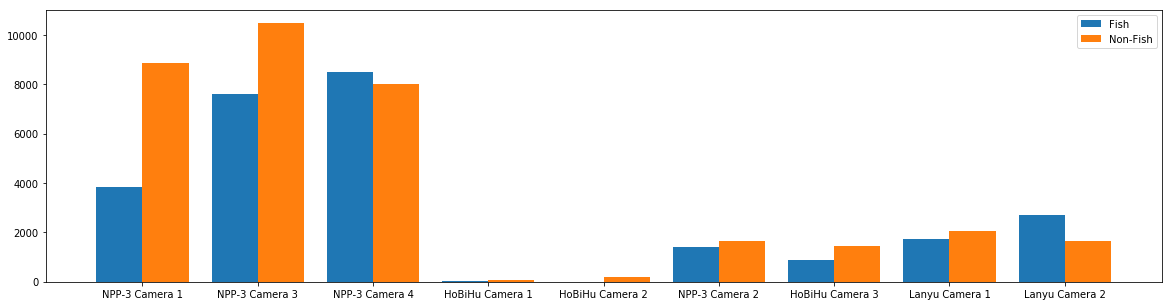
\includegraphics[scale=0.34]{graph/classdist.png}
    \caption{Number of Fish/Non-Fish at different sites in original Ground Truth Dataset}
    \label{fig:gtdist}
\end{figure}

Due to \DIFaddbegin \DIFadd{the }\DIFaddend need for re-calibration and future validation. 
Two \DIFdelbegin \DIFdel{separate subset }\DIFdelend \DIFaddbegin \DIFadd{additional subsets }\DIFaddend of videos, containing a total of 18,000 detections were marked.

\chapter{Preprocessing}
\label{chap:prepro}

\DIFdelbegin \DIFdel{While the data source problem is solved, the most costly part of the pipeline will be the feature extraction for the SVM part. 
It's not sensible to send all of the RGB values of a image as direct input for the SVM, hence feature extraction and dimensionality reduction is needed.
}%DIFDELCMD < 

%DIFDELCMD < %%%
\DIFdelend To achieve the goal of removing False Positives without losing too many True Positives, \DIFdelbegin \DIFdel{some }\DIFdelend \DIFaddbegin \DIFadd{as well as reducing the total runtime, some dataset }\DIFaddend reduction methods are used on the dataset before extraction of the features\DIFdelbegin \DIFdel{. 
Early Video Removal was introduced and an improved version of Frame Edge Indicator Function developed by Pugh was used.
}\DIFdelend \DIFaddbegin \DIFadd{: 
}\DIFaddend 

\DIFdelbegin \section{\DIFdel{Translation from MATLAB to Python}}
%DIFAUXCMD
\addtocounter{section}{-1}%DIFAUXCMD
%DIFDELCMD < \label{sec:translate}
%DIFDELCMD < %%%
\DIFdelend \DIFaddbegin \begin{itemize}
\setlength{\parskip}{1pt}
\item \textbf{\DIFadd{Early Video Removal}} \DIFadd{- Mark all detections recorded during night as Non-Fish.
}\item \textbf{\DIFadd{Frame Edge Indicator Function}}\DIFadd{, originally developed by Pugh\mbox{%DIFAUXCMD
\cite{Pugh} }%DIFAUXCMD
- Marking detections with a percentage of contour points touching the edge as Non-Fish. 
}\end{itemize}
\DIFaddend 

\DIFdelbegin \DIFdel{Initially the project aims to translate the entire pipeline into Python, however when it comes to the feature extraction part, translating the code became an unreasonable solution.
}\DIFdelend \DIFaddbegin \DIFadd{The next part of the pipeline will be the preprocessing stages:
}\DIFaddend 

\DIFdelbegin \DIFdel{The F4K feature extraction code have about 5, 000 lines of code in MATLAB.
Usually, for most of the MATLAB functions, an equivalent library function from Numpy/Scipy/SKLearn could be found.
Unfortunately, most of F4K feature extraction consists of customized code that could not be directly translated to Python.
}%DIFDELCMD < 

%DIFDELCMD < %%%
\DIFdel{For example, the Gabor Filter used in the project are written by Ahmad Poursaberi from Tehran University, a different implementation (where the scale of the filter is rotated, while their variance isn't) is used. 
This essentially required the project to re-engineer the whole F4K feature library.
}%DIFDELCMD < 

%DIFDELCMD < %%%
\DIFdel{A full translation of the F4K feature could take a few weeks. Since the cleaning algorithm only need to execute once, translation may not be the optimal path to take. After recording performance on various parts of the algorithm, we determined that one of the slowest operation is 2D convolution.
}%DIFDELCMD < 

%DIFDELCMD < \begin{figure}[h]
%DIFDELCMD <     \centering
%DIFDELCMD <     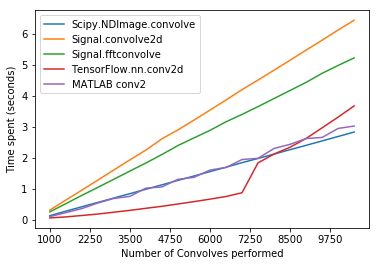
\includegraphics[scale=0.5]{graph/benchmark.png}
%DIFDELCMD <     %%%
%DIFDELCMD < \caption{%
{%DIFAUXCMD
\DIFdelFL{Test runtime of different 2D convolve algorithms.}}
    %DIFAUXCMD
%DIFDELCMD < \label{fig:benchmark}
%DIFDELCMD < \end{figure}
%DIFDELCMD < 

%DIFDELCMD < %%%
\DIFdel{Figure \ref{fig:benchmark} shows the tested performance of various 2D convolution algorithm.
During the test, 2000 random 100x100 arrays are generated to simulate images used, and 5 random 5x5 filters are used, simulating both the Gabor Filter and CNN usedin the pipeline. 
By enforcing the maximum computational thread to 1, the result shows that only 2 of the chosen algorithms in Python are faster than MATLAB.
}\DIFdelend \begin{itemize}
\DIFaddbegin \setlength{\parskip}{1pt}
\DIFaddend \item \DIFdelbegin \DIFdel{TensorFlow's conv2d, while faster than all other library, it has a significantly higher memory usage due to the tensor data type. It also have a high initialization cost due to the transformation needed.
}\DIFdelend \DIFaddbegin \textbf{\DIFadd{Feature extraction}} \DIFadd{and }\textbf{\DIFadd{dimensionality reduction}} \DIFadd{for the SVM classifier.
}\DIFaddend \item \DIFdelbegin \DIFdel{Scipy.NDImage's convolve, giving almost same performance as MATLAB.
}\DIFdelend \DIFaddbegin \textbf{\DIFadd{Colour space transformation}} \DIFadd{and }\textbf{\DIFadd{normalization}} \DIFadd{for the images CNN used. 
}\DIFaddend \end{itemize}

\DIFdelbegin \DIFdel{After this analysis, it's clear that re-engineering the MATLAB code is likely to spend more time, so a library called PyMatlab will be used to compute the F4K features in a MATLAB session instead, while other unfinished parts of the pipeline will be translated to Python.
}%DIFDELCMD < 

%DIFDELCMD < %%%
\DIFdelend \section{Early Video Removal}
\label{sec:earlyremove}

During the feature extraction tests, it \DIFdelbegin \DIFdel{is }\DIFdelend \DIFaddbegin \DIFadd{was }\DIFaddend discovered that loading a 40,000 frame video and \DIFdelbegin \DIFdel{extract }\DIFdelend \DIFaddbegin \DIFadd{extracting }\DIFaddend features from it would \DIFdelbegin \DIFdel{take }\DIFdelend \DIFaddbegin \DIFadd{use }\DIFaddend about 8 GB of memory space. 
\DIFdelbegin \DIFdel{If }\DIFdelend \DIFaddbegin \DIFadd{And if }\DIFaddend such video is processed on a node with RAM less than 8 GB, it will cause \DIFdelbegin \DIFdel{serious thrashing }\DIFdelend \DIFaddbegin \DIFadd{thrashing problems}\DIFaddend , rendering the \DIFdelbegin \DIFdel{node unresponsive. 
For machines having a RAM higher than 8 GB, it will still causes some disruption during loading}\DIFdelend \DIFaddbegin \DIFadd{machine unresponsive. 
It could still cause serious disruption on machines with higher RAM}\DIFaddend .

\DIFaddbegin \begin{figure}[ht]
\centering
    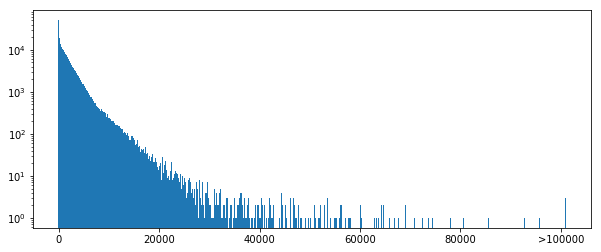
\includegraphics[scale=0.40]{graph/frame_distribution.png}
    \caption{\DIFaddFL{Log Scale Histogram of Detection Length}}
    \label{fig:vidlength}
\end{figure}

\DIFaddend While risking the chance of thrashing, these videos \DIFdelbegin \DIFdel{took }\DIFdelend \DIFaddbegin \DIFadd{will take }\DIFaddend a longer time to process, and most importantly, they are usually filled with \DIFdelbegin \DIFdel{False Positive }\DIFdelend \DIFaddbegin \DIFadd{Non-Fish }\DIFaddend detections. 
As discussed in Chapter \ref{sec:summaries}, if a camera recorded 30,000 \DIFdelbegin \DIFdel{detection }\DIFdelend \DIFaddbegin \DIFadd{detections }\DIFaddend in 10 minutes, means that in every frame of the original video, an average of 10 \DIFdelbegin \DIFdel{detection }\DIFdelend \DIFaddbegin \DIFadd{detections }\DIFaddend is extracted. 
\DIFaddbegin \DIFadd{Fig \ref{fig:vidlength} shows the Log Distribution of the videos with different length, note that only a few videos having detections more than 30,000. 
}\DIFaddend By looking at these \DIFdelbegin \DIFdel{"outlier" }\DIFdelend \DIFaddbegin \DIFadd{``outlier'' }\DIFaddend videos, some patterns were found \DIFaddbegin \DIFadd{(Images of these case are in Appendix \ref{append:samplelong})}\DIFaddend :

\begin{itemize}
\item
Both cameras at Lanyu site are night-vision cameras. When they film during the night, a lot of light \DIFdelbegin \DIFdel{reflecting }\DIFdelend \DIFaddbegin \DIFadd{is reflected from }\DIFaddend planktons and small animals close to the camera are recognised as fishes. Videos filmed during \DIFaddbegin \DIFadd{the }\DIFaddend night have an average of 6974 detections. 
\DIFdelbegin \DIFdel{A }\DIFdelend 5\% of the total \DIFdelbegin \DIFdel{detection comes }\DIFdelend \DIFaddbegin \DIFadd{detections come }\DIFaddend from such videos\DIFdelbegin \DIFdel{, with the }\DIFdelend \DIFaddbegin \DIFadd{. 
With a }\DIFaddend high False Positive rate, these videos can be safely excluded from cleaning.
\item
Videos full of compression/transmission errors \DIFdelbegin \DIFdel{, }\DIFdelend mostly happened at NPP-3 site camera 2 during June 2012 to August 2012. The camera falls down and \DIFdelbegin \DIFdel{change }\DIFdelend \DIFaddbegin \DIFadd{changed }\DIFaddend angles every few days. Even if there are no such errors, most of the detections are from moving background vegetation.
\item
One outlier video had 200,000 detections, consisting of lots of repeating frames, possibly caused by bugs in previous extraction processes.
\end{itemize}
There are also some good videos with high detections: 
\begin{itemize}
\item
Videos from NPP-3 site camera 3, at January 2010. These videos are captured at a higher frame rate, resulting in more \DIFdelbegin \DIFdel{detections. They usually contains lots of }\DIFdelend good detections.
\item
Dynamic background - Videos filled with moving vegetation, or refraction of sunlight. They usually \DIFdelbegin \DIFdel{contains }\DIFdelend \DIFaddbegin \DIFadd{contain }\DIFaddend lots of good detections.
\end{itemize}

\DIFdelbegin %DIFDELCMD < \begin{figure}[h]
%DIFDELCMD < \centering
%DIFDELCMD <     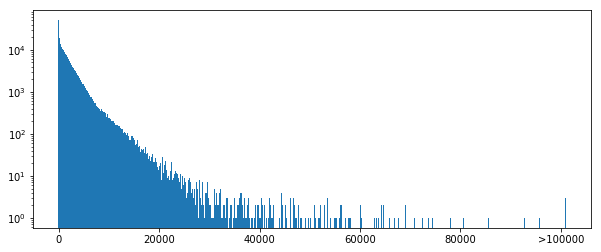
\includegraphics[scale=0.40]{graph/frame_distribution.png}
%DIFDELCMD <     %%%
%DIFDELCMD < \caption{%
{%DIFAUXCMD
\DIFdelFL{Log Scale Histogram of Detection Length}}
    %DIFAUXCMD
%DIFDELCMD < \label{fig:vidlength}
%DIFDELCMD < \end{figure}
%DIFDELCMD < 

%DIFDELCMD < %%%
\DIFdel{Using the above patterns and observed distribution in Fig \ref{fig:vidlength}, if }\DIFdelend \DIFaddbegin \DIFadd{If }\DIFaddend we remove all the videos recorded in the night, videos with 40,000 or more frames, and video recorded with above characteristics and 20,000 or more frames. About 8\% of the detections can be rejected without \DIFaddbegin \DIFadd{the }\DIFaddend need to extract them, saving approximately 200 days of computational time.
%Samples of rejected videos are in Appendix \ref{sec:samplelong}.

\section{Frame Edge Indicator Function (FEIF)}

In Pugh's thesis\cite{Pugh}, the FEIF is used to identify if a fish is being partially cut by the frame. 
In FEIF, \DIFdelbegin \DIFdel{a boundary of video is defined, and if the }\DIFdelend \DIFaddbegin \DIFadd{the boundary of the video like in Fig \ref{fig:feifzone} is used, the time-stamp zone comes from the reject area of the previous species recognition algorithm. 
If the }\DIFaddend number of the contour points \DIFdelbegin \DIFdel{outside of the boundary }\DIFdelend \DIFaddbegin \DIFadd{inside this zone }\DIFaddend exceeds 25, the detection is then rejected.

However\DIFaddbegin \DIFadd{, }\DIFaddend this function could not achieve the intention \DIFdelbegin \DIFdel{on some cases, for }\DIFdelend \DIFaddbegin \DIFadd{in some cases. 
For }\DIFaddend example, some videos have a darker frame edge, so even if a fish is cut by \DIFdelbegin \DIFdel{boundary, the contour points will be inside the boundary}\DIFdelend \DIFaddbegin \DIFadd{the boundary, it could still be accepted}\DIFaddend . 
Also, a large fish slightly touching the boundary will be rejected because the 25 limit \DIFdelbegin \DIFdel{, }\DIFdelend and small fishes may bypass the heuristics because of the size.

\DIFdelbegin \DIFdel{Following }\DIFdelend \DIFaddbegin \DIFadd{The following }\DIFaddend modification is added to solve the problem, by \DIFdelbegin \DIFdel{shrinking the boundary by }\DIFdelend \DIFaddbegin \DIFadd{padding the boundary for a }\DIFaddend 2 pixels \DIFaddbegin \DIFadd{width}\DIFaddend , then increasing the limit of 25 to 40, and adding a new restriction: reject all the detections with 25\% of the points touching the boundary. \DIFdelbegin \DIFdel{About 15}\DIFdelend %DIF > About 15\% of the dataset is rejected by this upgraded FEIF algorithm, saving 400 days of computational time.
\DIFaddbegin 

\begin{figure}[h]
\centering
    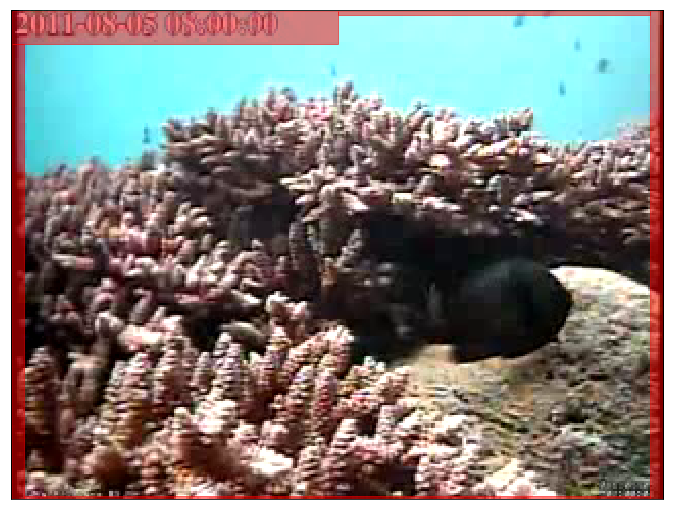
\includegraphics[scale=0.24]{graph/feifzone.png}
    \caption{\DIFaddFL{Removed Areas (highlighted with red colour) of the modified FEIF}}
    \label{fig:feifzone}
\end{figure}

\section{\DIFadd{Remove Rate of Reduction Algorithms}}
\label{sec:reduction}

\DIFadd{After testing the dataset reduction function on training dataset, the accuracy statistics below were obtained. This manages to remove about 40}\DIFaddend \% of the \DIFdelbegin \DIFdel{dataset is rejected by this upgraded FEIF algorithm}\DIFdelend \DIFaddbegin \DIFadd{bad detections, with about 5-10\% of False Negatives. It is later discovered to be the time-stamp setting problem, where a significant amount of fish gets rejected on videos without the time stamp. More details on the fault is in Section \ref{sec:feiffault}.
}


\newcolumntype{C}{>$c<$}
\begin{center}
\begin{tabular}{|c|c|c|}
\hline 
\DIFadd{$ $ }& \DIFadd{EVR and FEIF kept }& \DIFadd{EVR and FEIF reject }\\
\hline 
\DIFadd{True Fish }& \DIFadd{3060 }& \DIFadd{152 }\\
\DIFadd{Non Fish }& \DIFadd{3303 }& \DIFadd{1440 }\\
\hline 
\end{tabular}
\end{center}

\section{\DIFadd{Translation from MATLAB to Python}}
\label{sec:translate}

\DIFadd{Initially, the project aimed to translate the entire pipeline into Python, however when it came to the feature extraction part, translating the code became an unreasonable solution.
}

\DIFadd{The F4K feature extraction code has about 5}\DIFaddend ,\DIFdelbegin \DIFdel{saving 400 days of computational time}\DIFdelend \DIFaddbegin \DIFadd{000 lines of code in MATLAB.
Usually, for most of the MATLAB functions, an equivalent library function from Numpy/Scipy/SKLearn could be found.
Unfortunately, most of F4K feature extraction functions developed by Huang\mbox{%DIFAUXCMD
\cite{Huang} }%DIFAUXCMD
consists of customized code that could not be directly translated to Python.
}

\DIFadd{For example, the Gabor Filter used in the project was written by Ahmad Poursaberi from Tehran University, a different implementation (where the scale of the filter is rotated, while their variance isn't) is used. 
This essentially required the project to re-write the whole F4K feature library.
A full translation of the F4K feature could take a few weeks. 
}

\DIFadd{Since the cleaning algorithm only needs to execute once, translation may not be the optimal path to take. 
For this purpose, some benchmarking were tested to see if translating could reduce enough runtime on the project.
}

\begin{figure}[h]
    \centering
    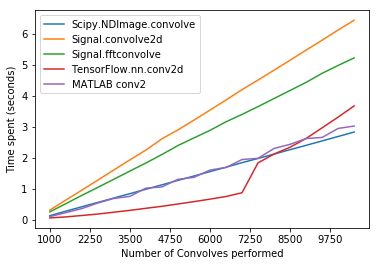
\includegraphics[scale=0.5]{graph/benchmark.png}
    \caption{\DIFaddFL{Test runtime of different 2D convolve algorithms.}}
    \label{fig:benchmark}
\end{figure}

\DIFadd{Figure \ref{fig:benchmark} shows the tested performance of various 2D convolution algorithm. During the test, 2000 random 100x100 arrays are generated to simulate images used, and 5 random 5x5 filters are used, simulating both the Gabor Filter and CNN used in the pipeline. By enforcing the maximum computational thread to 1, the result shows that only 2 of the chosen algorithms in Python are faster than MATLAB.
}\begin{itemize}
\setlength{\parskip}{1pt}
\item
\textbf{\DIFadd{TensorFlow's conv2d}}\DIFadd{, while faster than all other libraries, it has a significantly higher memory usage due to the use of tensor data type. Translation using this would be difficult due to the library being focused on Neural Networks.
}\item
\textbf{\DIFadd{Scipy.NDImage's convolve}}\DIFadd{, giving an almost same performance as MATLAB.
}\end{itemize}

\DIFadd{After this analysis, it's clear that re-engineering the MATLAB code is likely to spend more time, so a library called PyMatlab will be used to compute the F4K features in a MATLAB session instead, while other unfinished parts of the pipeline will be translated to Python}\DIFaddend .

\section{Feature Extraction}

During the species recognition stage of the F4K project, 2626 features were used for computing \DIFaddbegin \DIFadd{the }\DIFaddend detection certainty.
On that basis, Pugh added 29 new features focused on the edges of the contour. 
\DIFdelbegin \DIFdel{Then }\DIFdelend \DIFaddbegin \DIFadd{After that, }\DIFaddend dimensionality reduction is applied to the features to reduce dimension from 2655 to 88.

This process takes about 0.3 seconds for each frame, Analysing the computational time shows the following result, sorted by time cost:
\begin{itemize}
\DIFaddbegin \setlength{\parskip}{1pt}
\DIFaddend \item
\DIFdelbegin \DIFdel{Co-occurance Matrix }\DIFdelend \DIFaddbegin \textbf{\DIFadd{Co-occurrence Matrix}} \DIFaddend - these 720 features took about 0.2 seconds to compute.
\item
\DIFdelbegin \DIFdel{Affine Moment Invariants }\DIFdelend \DIFaddbegin \textbf{\DIFadd{Affine Moment Invariants}} \DIFaddend - these 105 features took 0.05 seconds to compute.
\item
\DIFdelbegin \DIFdel{Gabor Filter }\DIFdelend \DIFaddbegin \textbf{\DIFadd{Gabor Filter}} \DIFaddend - these 160 features took about 0.04 seconds to compute.
\item \DIFdelbegin \DIFdel{Rest of the features took }\DIFdelend \DIFaddbegin \DIFadd{Other features took an }\DIFaddend almost negligible amount of time to finish.
\end{itemize}
Unfortunately\DIFaddbegin \DIFadd{, }\DIFaddend after checking the features with PCA, these feature all took \DIFaddbegin \DIFadd{a }\DIFaddend significant part in the first 50 PCA components, removing any one of \DIFdelbegin \DIFdel{the 3 }\DIFdelend \DIFaddbegin \DIFadd{these }\DIFaddend time costly feature will have a high impact on the result.

\DIFaddbegin \subsection{\DIFadd{Huang's Features}}

\DIFadd{Pugh's work was based on the previous work of Huang's\mbox{%DIFAUXCMD
\cite{Huang}}%DIFAUXCMD
, where his 2626 features were used to identify the species of a fish.
Since this part is not translated, only a list of used feature are provided here:
}\begin{itemize}
\setlength{\parskip}{1pt}
\item \textbf{\DIFadd{RGB and HSV histograms}} \DIFadd{- 930 features.
}\item \textbf{\DIFadd{Curve Tail Shape, Ratio}} \DIFadd{- 2 features.
}\item \textbf{\DIFadd{Fish Density Static}} \DIFadd{- 12 features.
}\item \textbf{\DIFadd{Co-occurance Matrix}} \DIFadd{- 720 features.
}\item \textbf{\DIFadd{Moment Invariant}} \DIFadd{- 42 features.
}\item \textbf{\DIFadd{Pyramid Histogram of Gradient}} \DIFadd{- 680 features.
}\item \textbf{\DIFadd{Fourier Descriptor}} \DIFadd{- 15 features.
}\item \textbf{\DIFadd{Gabor Filter on Textures}} \DIFadd{- 160 features.
}\item \textbf{\DIFadd{Affine Moment Invariants}} \DIFadd{- 63 features.
}\item \textbf{\DIFadd{Tail/Head Contour Point Ratio}} \DIFadd{- 2 features.
}\end{itemize}

\DIFaddend \subsection{Pugh's Features}

Pugh's part of the generated \DIFdelbegin \DIFdel{feature consist }\DIFdelend \DIFaddbegin \DIFadd{features consists }\DIFaddend of 4 parts: Animation Score, Boundary Curvature, Erraticity, and Gabor Filter on \DIFdelbegin \DIFdel{edge}\DIFdelend \DIFaddbegin \DIFadd{contours}\DIFaddend . 
This part of the pipeline is translated into Python as the original feature generation script is incomplete. Some inefficient {\tt for} loops were translated using \DIFdelbegin \DIFdel{Numpy library to speed them up}\DIFdelend \DIFaddbegin \DIFadd{the Numpy library for maximal single-core performance}\DIFaddend .

\DIFdelbegin \DIFdel{The Animation Score (AS) }\DIFdelend \DIFaddbegin \begin{itemize}
\setlength{\parskip}{1pt}
\item
\textbf{\DIFadd{Animation Score (AS)}} \DIFaddend is calculated for one whole track, where 5 frames are \DIFdelbegin \DIFdel{pick }\DIFdelend \DIFaddbegin \DIFadd{picked }\DIFaddend from the track \DIFdelbegin \DIFdel{, }\DIFdelend and squared sum of the change in pixels is calculated. This feature isn't very useful because of the dynamic background of the image.
\DIFdelbegin %DIFDELCMD < 

%DIFDELCMD < %%%
\DIFdel{Boundary Curvature (BC), it }\DIFdelend \DIFaddbegin \item
\textbf{\DIFadd{Boundary Curvature (BC)}}\DIFadd{, }\DIFaddend uses the Curvature Scale Space to measure the change of direction to the contour, the result is blurred with a Gaussian filter and the Skewness and Kurtosis is extracted. 
\DIFdelbegin %DIFDELCMD < 

%DIFDELCMD < %%%
\DIFdel{Temporal Consistency (Erraticity) }\DIFdelend \DIFaddbegin \item
\textbf{\DIFadd{Temporal Consistency (Erraticity)}} \DIFaddend is similar to Boundary Curvature, where 5 frames are picked and mean of Skewness and Kurtosis is recorded.
\DIFdelbegin %DIFDELCMD < 

%DIFDELCMD < %%%
\DIFdel{Gabor Filters }\DIFdelend \DIFaddbegin \item
\textbf{\DIFadd{Gabor Filters}} \DIFaddend applied on binary \DIFdelbegin \DIFdel{image }\DIFdelend \DIFaddbegin \DIFadd{images }\DIFaddend generated using contour, instead of the original image used in the F4K feature extraction. 
\DIFaddbegin \end{itemize}
\DIFaddend 

\subsection{Principle Component Analysis}

Originally in Pugh's design, the number of the Principle Components used were selected with Kaiser's Criterion, where only ones with \DIFaddbegin \DIFadd{an }\DIFaddend eigenvalue greater than 1 \DIFdelbegin \DIFdel{is }\DIFdelend \DIFaddbegin \DIFadd{are }\DIFaddend selected. 
However\DIFaddbegin \DIFadd{, }\DIFaddend the only advantage with this criterion is it \DIFdelbegin \DIFdel{being }\DIFdelend \DIFaddbegin \DIFadd{is }\DIFaddend easy to calculate, essentially throwing away 30\% of \DIFdelbegin \DIFdel{informations. }\DIFdelend \DIFaddbegin \DIFadd{the information. This loss could be directly observed from Fig \ref{fig:pcsused}.
}\DIFaddend 

Also due to \DIFdelbegin \DIFdel{storages }\DIFdelend \DIFaddbegin \DIFadd{the storage }\DIFaddend limit of the project, about 100 features per frame could be stored. With this problem, the first 88 Principle Components were used, this \DIFdelbegin \DIFdel{express }\DIFdelend \DIFaddbegin \DIFadd{expresses }\DIFaddend 90\% of the variance of the training dataset.

\begin{figure}[ht]
\centering
    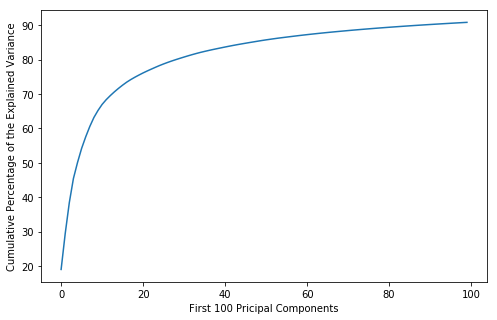
\includegraphics[scale=0.40]{graph/pcas.png}
    \caption{\DIFaddbeginFL \DIFaddFL{Cumulative }\DIFaddendFL Variance Explained \DIFaddbeginFL \DIFaddFL{against Number of Features Used}\DIFaddendFL }
    \label{fig:pcsused}
\end{figure}

\section{Image Processing For CNN}
\label{sec:CNNprepro}

In Pugh's pipeline classifier, 3 different CNNs were used on \DIFdelbegin \DIFdel{different type }\DIFdelend \DIFaddbegin \DIFadd{the different types }\DIFaddend of preprocessed images.
In  {\tt CNN\_N}, \DIFaddbegin \DIFadd{the }\DIFaddend normal image is used, in {\tt CNN\_WC} and {\tt CNN\_BC}, a masked image is used, filling the pixels outside the contour with white and black respectively.
For the BC and WC images, \DIFdelbegin \DIFdel{it }\DIFdelend \DIFaddbegin \DIFadd{the detection }\DIFaddend is then moved to \DIFdelbegin \DIFdel{center }\DIFdelend \DIFaddbegin \DIFadd{the centre }\DIFaddend of the image.

Before the image is \DIFdelbegin \DIFdel{forward }\DIFdelend \DIFaddbegin \DIFadd{input }\DIFaddend into the CNN\DIFdelbegin \DIFdel{models}\DIFdelend , transformation and normalization is performed. 
Firstly the image is transformed into YUV \DIFdelbegin \DIFdel{color }\DIFdelend \DIFaddbegin \DIFadd{colour }\DIFaddend space.
Then the image is normalized globally with \DIFaddbegin \DIFadd{the }\DIFaddend mean and standard deviation of the YUV images.
Finally, local spatial normalization was applied \DIFdelbegin \DIFdel{on }\DIFdelend \DIFaddbegin \DIFadd{to }\DIFaddend each channel.
\DIFaddbegin \DIFadd{This process is shown in Fig \ref{fig:imageprepro}.
}\DIFaddend 

\DIFdelbegin \DIFdel{However after }\DIFdelend \DIFaddbegin \begin{figure}[ht]
\centering
    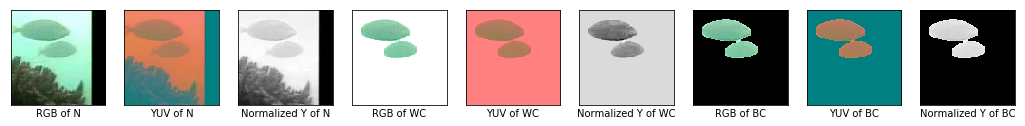
\includegraphics[scale=0.4]{graph/imagepre.png}
    \caption{\DIFaddFL{Images on first stages of pre-process}}
    \label{fig:imageprepro}
\end{figure}

\DIFadd{After }\DIFaddend tests on the \DIFdelbegin \DIFdel{CNN trained , the result }\DIFdelend \DIFaddbegin \DIFadd{trained CNNs, the results }\DIFaddend obtained weren't even close to the ones Pugh obtained.
It \DIFdelbegin \DIFdel{is }\DIFdelend \DIFaddbegin \DIFadd{was }\DIFaddend discovered that during the preprocessing stage of Pugh, two major mistakes were made \DIFdelbegin \DIFdel{.
Pughuses }\DIFdelend \DIFaddbegin \DIFadd{due to Pugh's usage of }\DIFaddend OpenCV's {\tt imwrite} for the extraction of the image\DIFdelbegin \DIFdel{, the }\DIFdelend \DIFaddbegin \DIFadd{.
}

\begin{itemize}
\setlength{\parskip}{1pt}
\item
\DIFadd{The }\DIFaddend images are stored in compressed {\tt \DIFdelbegin \DIFdel{".jpeg"}\DIFdelend \DIFaddbegin \DIFadd{``.jpeg''}\DIFaddend } format, this leads to \DIFaddbegin \DIFadd{a }\DIFaddend drastic change in the result matrix, due to the local normalization step. 
\DIFaddbegin \item
\DIFaddend Another fatal mistake is the \DIFdelbegin \DIFdel{image store }\DIFdelend \DIFaddbegin \DIFadd{images stored }\DIFaddend with OpenCV are in BGR space, where Lua recognize it as \DIFaddbegin \DIFadd{an }\DIFaddend RGB image.
\DIFdelbegin %DIFDELCMD < 

%DIFDELCMD < %%%
\DIFdelend \DIFaddbegin \end{itemize}
\DIFaddend This causes the CNN\_N and CNN\_BC almost useless, classifying almost every unseen data into 1 single class. Some re-train attempt were included in Section \ref{sec:cnn}.

\DIFdelbegin %DIFDELCMD < \begin{figure}[h]
%DIFDELCMD < \centering
%DIFDELCMD <     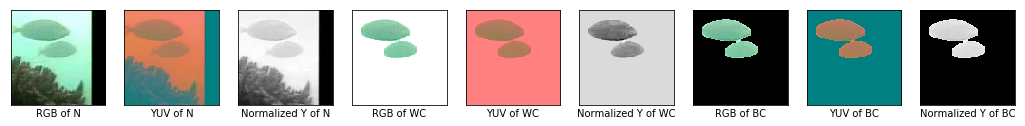
\includegraphics[scale=0.4]{graph/imagepre.png}
%DIFDELCMD <     %%%
%DIFDELCMD < \caption{%
{%DIFAUXCMD
\DIFdelFL{Images on first stages of pre-process}}
    %DIFAUXCMD
%DIFDELCMD < \label{fig:imageprepro}
%DIFDELCMD < \end{figure}
%DIFDELCMD < %%%
\DIFdelend \DIFaddbegin \DIFadd{Half of the cleaning time cost comes from the image normalization of the CNN in the original pipeline design.
With optimizations applied at the translation stage, the time cost for the pre-processing is drastically reduced to 3 days. 
This reduction is done by removing of SQL server and translated MATLAB normalization code in Python.
}\DIFaddend 



\chapter{Classification}
\label{chap:classify}

\section{Ambiguity in Original Classification Schema}
\label{sec:AmbigCS}

For the Pipeline Classifier, 10 \DIFdelbegin \DIFdel{classes of different }\DIFdelend \DIFaddbegin \DIFadd{different 1classes of }\DIFaddend detections were proposed in Section \ref{sec:schema}, but there are many limitations on this schema.
For example, some cases could be appearing simultaneously\DIFdelbegin \DIFdel{, a detection }\DIFdelend \DIFaddbegin \DIFadd{. Detection }\DIFaddend could have an erratic boundary, and also touching the boundary of a frame. Pugh's thesis didn't state clearly \DIFdelbegin \DIFdel{different priority }\DIFdelend \DIFaddbegin \DIFadd{the different priorities }\DIFaddend among classes used. 

After looking through the previously marked ground truth data, it is also found that some classes are very similar to others. For example in Fig \ref{fig:class68}, the track has a detection contour that is progressively less erratic. It makes it hard to draw an exact boundary between different classes when classifying manually.

\begin{figure}[h]
\centering
    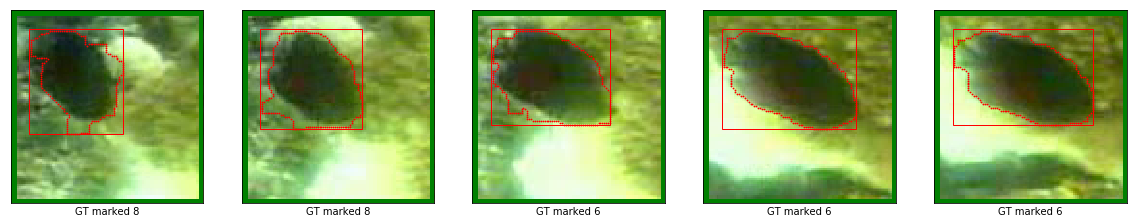
\includegraphics[scale=0.34]{graph/6-8.png}
    \caption{Detection changing from class 8 (Bad Boundary) to 6 (Clean Boundary).}
    \label{fig:class68}
\end{figure}

Another example of this is shown in Fig \ref{fig:class56}, where initially it is unknown whether the detection is a fish or not given the single frame. This is more problematic because the extraction intends to throw away class 5 while \DIFdelbegin \DIFdel{keep }\DIFdelend \DIFaddbegin \DIFadd{keeping }\DIFaddend class 6 detections. 

\begin{figure}[ht]
\centering
    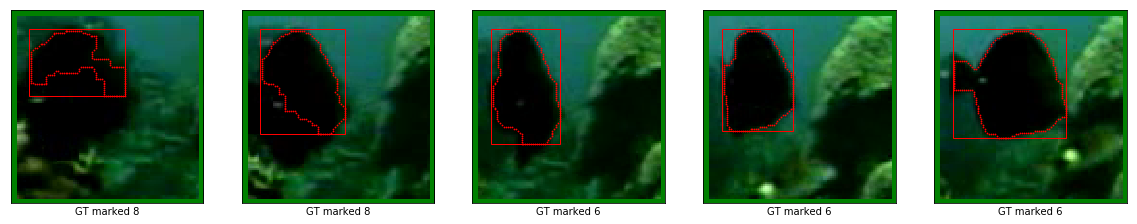
\includegraphics[scale=0.34]{graph/5-6.png}
    \caption{A track of detection, changing from class 5 (Unknown) to 6 (Fish).}
    \label{fig:class56}
\end{figure}

Similar problem \DIFdelbegin \DIFdel{has }\DIFdelend \DIFaddbegin \DIFadd{have }\DIFaddend also occurred between \DIFdelbegin \DIFdel{\(class\in[2,3,4,5,8,6]\)}\DIFdelend \DIFaddbegin \DIFadd{\(classes\in[2,3,4,5,8,6]\)}\DIFaddend . Where class 2, 3, and 4 generally means \DIFdelbegin \DIFdel{"}\DIFdelend \DIFaddbegin \DIFadd{``}\DIFaddend I'm not sure what this is, but it's definitely not a fish\DIFdelbegin \DIFdel{"}\DIFdelend \DIFaddbegin \DIFadd{''}\DIFaddend , and on the other side, class 6 represents fish with good detection boundary. 
Also, any one of the \DIFdelbegin \DIFdel{detection }\DIFdelend \DIFaddbegin \DIFadd{detections }\DIFaddend might suddenly change to class 7 (partial fish visible) just because they are close to the frame edge. 

For the \DIFdelbegin \DIFdel{case }\DIFdelend \DIFaddbegin \DIFadd{cases }\DIFaddend of class 2 and 3, they are errors captured by the F4K species extraction's background removal issues, caused by illumination and background vegetation respectively.
During the ground truth \DIFdelbegin \DIFdel{process }\DIFdelend \DIFaddbegin \DIFadd{processing }\DIFaddend of new datasets, it is found that \DIFdelbegin \DIFdel{distinguish }\DIFdelend \DIFaddbegin \DIFadd{distinguishing }\DIFaddend between these two \DIFdelbegin \DIFdel{class are }\DIFdelend \DIFaddbegin \DIFadd{classes is almost }\DIFaddend impossible.
This indicates that confusion matrix might not be a good indicator whether a classifier performs well or not. In fact, if the classifier performs too well, it would indicate the classifier over-fits on the training dataset instead.

The original goal of the project is to remove non-fish detections from the dataset, hence only fish marked with class 6 and 8 are kept\DIFdelbegin \DIFdel{, it }\DIFdelend \DIFaddbegin \DIFadd{. 
It }\DIFaddend is more tolerable for \DIFdelbegin \DIFdel{"}\DIFdelend \DIFaddbegin \DIFadd{``}\DIFaddend fish-like\DIFdelbegin \DIFdel{" }\DIFdelend \DIFaddbegin \DIFadd{'' }\DIFaddend classes like class 9 (Fish with Error) and class 7 (Partial visible) to be classified as fish.
On the other hand, class 1 (Compression Fault) classified as class 6 (Good Fish) needed to be penalized heavily. 

With this addition to accuracy metrics, the SVM and CNN developed by Pugh \DIFdelbegin \DIFdel{were evaluated again}\DIFdelend \DIFaddbegin \DIFadd{was re-evaluated}\DIFaddend , and unfortunately, both \DIFdelbegin \DIFdel{need rework for it }\DIFdelend \DIFaddbegin \DIFadd{needed rework }\DIFaddend to work properly again.

\section{Support Vector Machines (SVM)}

In the original design, Pugh \DIFdelbegin \DIFdel{uses }\DIFdelend \DIFaddbegin \DIFadd{used }\DIFaddend ten different SVM \DIFdelbegin \DIFdel{classifier }\DIFdelend \DIFaddbegin \DIFadd{classifiers }\DIFaddend with RBF kernel (Radial Basis Function kernel) for \DIFdelbegin \DIFdel{marking }\DIFdelend \DIFaddbegin \DIFadd{estimating }\DIFaddend probability of each class. Each of the \DIFdelbegin \DIFdel{SVM }\DIFdelend \DIFaddbegin \DIFadd{SVMs }\DIFaddend has a parameter setting of:
\DIFdelbegin %DIFDELCMD < \renewcommand{\labelenumi}{\arabic{enumi}}
%DIFDELCMD < %%%
\DIFdelend \DIFaddbegin \renewcommand{\labelenumi}{\bfseries\arabic{enumi}}
\DIFaddend \begin{enumerate}
\DIFaddbegin \setlength{\parskip}{1pt}
	\DIFaddend \item In the Kernel Function \(K(x,x') = exp(-\gamma\norm{x-x'}^2)\), a \(\gamma\) value around 4-5.
	\item Soft Margin Parameter C set to 1.
\end{enumerate}
Translating the SVM design to python is trivial, the package {\tt sklean.svm} provides a easy-to-use implement of the SVM, with only the need to fit the dataset again.
The only different between MATLAB and Python's SVM is the parameter \(\gamma\) used, Python use \(\sigma\) for rbf kernel. A simple translation could be used to find the corresponding \(\sigma\) value, using the formula \( \gamma = 1/2\sigma^2 \).

In Pugh's design, due to the limitations of an incomplete training dataset, the result is heavily biased. After testing on unseen data, it classifies almost every detection as class 7 (partial fish visible). In order to fully utilize the features extracted, another search \DIFdelbegin \DIFdel{of parameter }\DIFdelend \DIFaddbegin \DIFadd{for parameters }\DIFaddend over C and \(\sigma\) is needed.

Pugh's search for optimal parameters involves finding \(\gamma\in[2^{-5},2^{-3}...2^{13},2^{15}]\) that gives the highest accuracy among the pre-split dataset, due to the \DIFdelbegin \DIFdel{amount }\DIFdelend \DIFaddbegin \DIFadd{number }\DIFaddend of features used and the size of the dataset, training a single SVM could take from \DIFdelbegin \DIFdel{30-minute to 2-hour}\DIFdelend \DIFaddbegin \DIFadd{30-minutes to 2-hours}\DIFaddend . Using the new grid search involving C and K-Folding, about 500 new SVM are needed to fit for finding the optimal value, \DIFdelbegin \DIFdel{it }\DIFdelend \DIFaddbegin \DIFadd{this }\DIFaddend would take over months to complete.
With the help of the task distribution system developed, it took about 4 hours to find the
new optimal \(\sigma = 10^{-3}\), and \(C = 1\).
The result of the SVM is shown in Fig \ref{fig:svmacc}.

\DIFaddbegin \DIFadd{Fig \ref{fig:svmacc} shows the confusion matrix of the result after testing it on the additional validation dataset, using the original top-N algorithm developed by Pugh\mbox{%DIFAUXCMD
\cite{Pugh}}%DIFAUXCMD
. 
At first, the result looks promising, but after normalizing it is shown that a high percentage of the detections is marked as class 7.
It is suspected that the classifier has learned class 7 as it's ``Base Case'', where every detection it doesn't know about is classified as class 7.
}

\DIFadd{Without this interference, the SVM could still obtain reasonable results.
Some attempt at removing this problem can be found in Section \ref{sec:voting}.
}

\DIFaddend \begin{figure}[h]
\centering
    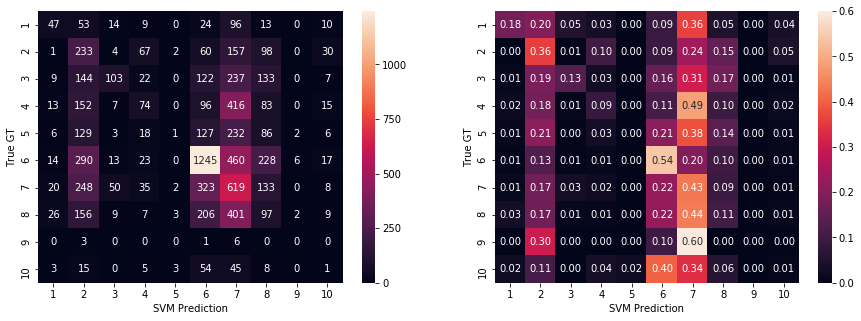
\includegraphics[scale=0.44]{graph/svmresult.png}
    \caption{SVM's result and normalized result on unseen dataset}
    \label{fig:svmacc}
\end{figure} 

\section{Convolutional Neural Networks (CNN)}
\label{sec:cnn}

%DIF < TODO voting link.
As mentioned before in Section \ref{sec:CNNprepro}, the result of the CNN were heavily affected by the preprocessing \DIFdelbegin \DIFdel{error. This causes the }\DIFdelend \DIFaddbegin \DIFadd{errors. This caused }\DIFaddend one of the CNN learning too many unnecessary and random features of the image, which produces a poor accuracy on the unseen dataset, marking almost every image it sees \DIFdelbegin \DIFdel{into }\DIFdelend \DIFaddbegin \DIFadd{as }\DIFaddend class 2 or \DIFdelbegin \DIFdel{7. 
%DIF < %%INSERTHERE
}\DIFdelend \DIFaddbegin \DIFadd{7 detections. 
}\DIFaddend 

However even under this fault, the CNN\_WC (CNN using \DIFaddbegin \DIFadd{an }\DIFaddend image with white mask) still manages to produce \DIFaddbegin \DIFadd{a }\DIFaddend reasonable result, and after testing different voting strategies, it's discovered that CNN\_BC (CNN using \DIFaddbegin \DIFadd{an }\DIFaddend image with black mask) could also contribute in \DIFaddbegin \DIFadd{the }\DIFaddend final classification.
\DIFaddbegin \DIFadd{This can be seen in Fig \ref{fig:cnnbcacc}, the class 7 problem in SVM can also be found in this graph.
}\DIFaddend 

\DIFaddbegin \begin{figure}[h]
\centering
    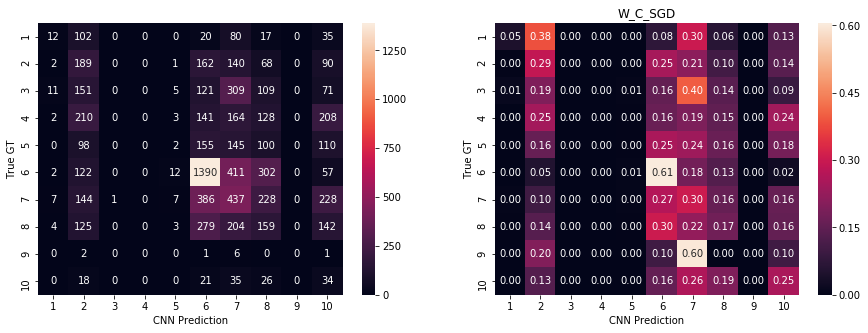
\includegraphics[scale=0.44]{graph/cnnwc.png}
    \caption{\DIFaddFL{CNN\_WC's result and normalized result on unseen dataset}}
    \label{fig:cnnbcacc}
\end{figure} 

\DIFaddend Since the classification gives a poor result compared to the accuracy achieved in Pugh's thesis\cite{Pugh}, it is first suspected that the translated Python code \DIFdelbegin \DIFdel{perform }\DIFdelend \DIFaddbegin \DIFadd{performed }\DIFaddend differently than the MATLAB's extraction.
After discussion with Pugh\DIFaddbegin \DIFadd{, }\DIFaddend he mentioned the extraction procedure \DIFdelbegin \DIFdel{were }\DIFdelend \DIFaddbegin \DIFadd{was }\DIFaddend different in his final pipeline.

His previous work uses MATLAB to experiment and evaluate on different classifiers\DIFdelbegin \DIFdel{, however  }\DIFdelend \DIFaddbegin \DIFadd{.
However, }\DIFaddend when it comes to the extraction process, Python's OpenCV library \DIFdelbegin \DIFdel{were }\DIFdelend \DIFaddbegin \DIFadd{was }\DIFaddend used instead of the MATLAB ones.
OpenCV stores \DIFdelbegin \DIFdel{a }\DIFdelend \DIFaddbegin \DIFadd{an }\DIFaddend image in BGR space by default, and Lua loads the extracted images in RGB.

Because of lacking a second set of validation data, the final training \DIFdelbegin \DIFdel{were }\DIFdelend \DIFaddbegin \DIFadd{was }\DIFaddend not validated, the mistake in \DIFdelbegin \DIFdel{color space is }\DIFdelend \DIFaddbegin \DIFadd{colour space was }\DIFaddend not noticed until this project actually uses the trained model.

At the time of the project\DIFdelbegin \DIFdel{it is considered the re-train }\DIFdelend \DIFaddbegin \DIFadd{, we considered re-training }\DIFaddend of a new model\DIFdelbegin \DIFdel{, the original model were }\DIFdelend \DIFaddbegin \DIFadd{. 
The original model was }\DIFaddend trained with CUDA support, \DIFdelbegin \DIFdel{were }\DIFdelend \DIFaddbegin \DIFadd{but }\DIFaddend the machine nodes used in this project \DIFdelbegin \DIFdel{does not have a }\DIFdelend \DIFaddbegin \DIFadd{do not have an }\DIFaddend NVIDIA video card. 
After evaluating Pugh's source code, each epoch of the training could take a full day on a single node, and \DIFdelbegin \DIFdel{re-train }\DIFdelend \DIFaddbegin \DIFadd{re-training }\DIFaddend with the current \DIFdelbegin \DIFdel{frame work }\DIFdelend \DIFaddbegin \DIFadd{framework }\DIFaddend would take 20 days on 200 machines, not to mention the disruption caused by the high memory usage. 
It \DIFdelbegin \DIFdel{is }\DIFdelend \DIFaddbegin \DIFadd{was }\DIFaddend also considered to apply for a specialized cluster for the \DIFdelbegin \DIFdel{re-train}\DIFdelend \DIFaddbegin \DIFadd{re-training}\DIFaddend , but due to the lack of time, re-train \DIFdelbegin \DIFdel{were }\DIFdelend \DIFaddbegin \DIFadd{was }\DIFaddend not used in this project.

\DIFdelbegin %DIFDELCMD < \begin{figure}[h]
%DIFDELCMD < \centering
%DIFDELCMD <     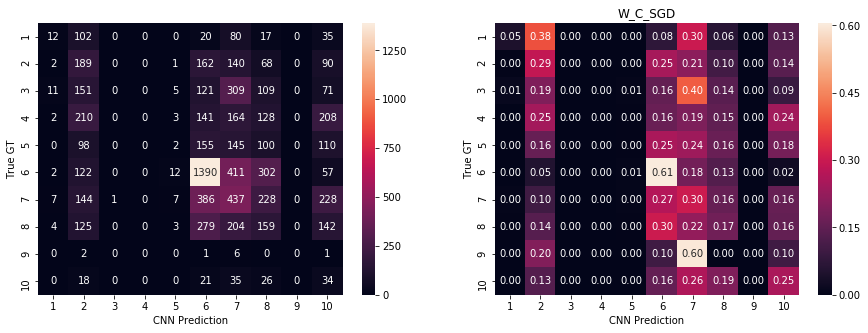
\includegraphics[scale=0.44]{graph/cnnwc.png}
%DIFDELCMD <     %%%
%DIFDELCMD < \caption{%
{%DIFAUXCMD
\DIFdelFL{CNN\_WC's result and normalized result on unseen dataset}}
    %DIFAUXCMD
%DIFDELCMD < \label{fig:cnnbcacc}
%DIFDELCMD < \end{figure} 
%DIFDELCMD < 

%DIFDELCMD < %%%
\DIFdelend %\begin{figure}[h]
%\centering
%    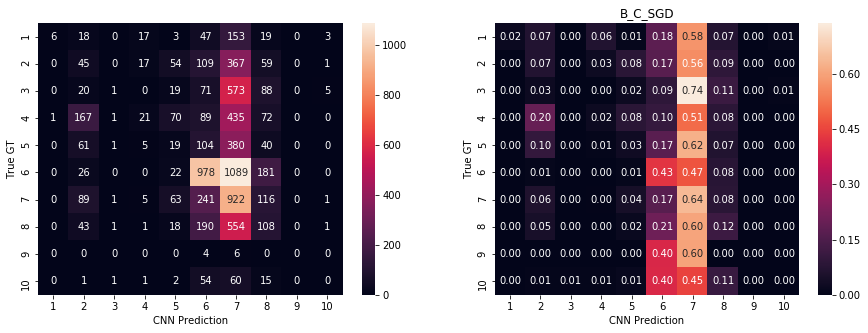
\includegraphics[scale=0.44]{graph/cnnbc.png}
%    \caption{CNN\_BC's result and normalized result on unseen dataset}
%    \label{fig:cnnwcacc}
%\end{figure} 

%\section{Evaluation}
%\section{Potential Candidate of classifiers}

%\chapter{Voting Strategy}
%\label{chap:voting}

\section{Voting Strategy}
\label{sec:voting}

As the classifier \DIFdelbegin \DIFdel{do }\DIFdelend \DIFaddbegin \DIFadd{does }\DIFaddend not work as expected as in Pugh's thesis, it is reconsidered to apply the previously failed attempts on increasing accuracy of the classifiers.
One of the \DIFdelbegin \DIFdel{method }\DIFdelend \DIFaddbegin \DIFadd{methods }\DIFaddend tested is to add a voting method on the predicted probabilities obtained by different classifiers, to test out different combination of the classifier results.

%DIF < \subsection{Evaluation of Yu's approach}
%DIF < In 2016, Yu\cite{Yu} tried to add voting constraint on the classifier and evaluated the %efficiency.
%DIF < Where Yu introduced a method of removing 
%DIF < However the voting strategy does not work as intended due to the following assumption:
%DIF < Yu's thesis explored three tracked-based voting methods, which removes a detection track entirely if less than 50\% of the detection is classified as non-fish.
\DIFaddbegin \DIFadd{The voting strategy is described in the pseudo-code below. 
The input: }{\tt \DIFadd{predict}} \DIFadd{is the predicted probability outputs of the classifiers, while the other parameters are the options used for searching the best combination of the classifiers. 
}\DIFaddend 

\DIFaddbegin \begin{center}
\vspace{10pt}
\textbf{\DIFadd{Code removed for generating diff.}}
\vspace{10pt}
\end{center}

\DIFadd{After testing through different settings, a Receiver Operating Characteristic (ROC) curve of the voting performance is plotted.
The ROC curve plotted is shown in Fig \ref{fig:roccurve}, this shows the True Positive Rate (good fish kept) against False Positive Rate (bad detections kept) at different thresholds ($\gamma$ value in the pseudo-code).
}

\begin{figure}[ht]
\centering
    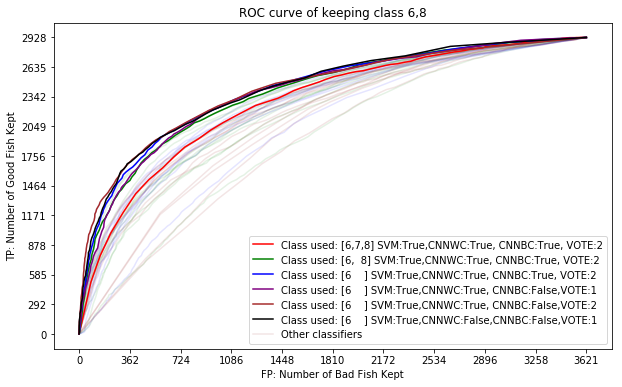
\includegraphics[scale=0.6]{graph/roccurve.png}
    \caption{\DIFaddFL{ROC curve of different settings for voting algorithm}}
    \label{fig:roccurve}
\end{figure} 

\DIFadd{The project can only afford to lose about 10\% of the good fish.
With this limit, the best classifier it to use SVM's predicted class 6 probability only, the ROC curve of this classifier is the black curve in Fig \ref{fig:roccurve}. 
}

\DIFadd{The chosen gamma value for the criteria is 0.0108, meaning all detection with SVM's class 6 probability higher than 1.1\% is classified as a fish.
After the method is tested on various datasets from ground truth, and the following statistics are obtained.
}

\begin{center}
\begin{tabular}{|c|c|c|c|c|}
\hline 
\DIFadd{$ $ Training Dataset }& \DIFadd{EVR reject }& \DIFadd{FEIF reject }& \DIFadd{SVM reject }& \DIFadd{Detection Kept}\\
\hline 
\DIFadd{True Fish }& \DIFadd{2858 }& \DIFadd{1090 }& \DIFadd{491 }& \DIFadd{26211 }\\
\DIFadd{Non Fish }& \DIFadd{1955 }& \DIFadd{10577 }& \DIFadd{7690 }& \DIFadd{19511 }\\
\hline 
\end{tabular}
\end{center}

\begin{center}
\begin{tabular}{|c|c|c|c|c|}
\hline 
\DIFadd{$ $ Validation Dataset 1 }& \DIFadd{EVR reject }& \DIFadd{FEIF reject }& \DIFadd{SVM reject }& \DIFadd{Detection Kept}\\
\hline 
\DIFadd{True Fish }& \DIFadd{61 }& \DIFadd{91 }& \DIFadd{88 }& \DIFadd{2972 }\\
\DIFadd{Non Fish }& \DIFadd{266 }& \DIFadd{1174  }& \DIFadd{553 }& \DIFadd{2750 }\\
\hline 
\end{tabular}
\end{center}

\begin{center}
\begin{tabular}{|c|c|c|c|c|}
\hline 
\DIFadd{$ $ Validation Dataset 2 }& \DIFadd{EVR reject }& \DIFadd{FEIF reject }& \DIFadd{SVM reject }& \DIFadd{Detection Kept}\\
\hline 
\DIFadd{True Fish }& \DIFadd{1 }& \DIFadd{13  }& \DIFadd{2 }& \DIFadd{373 }\\
\DIFadd{Non Fish }& \DIFadd{38 }& \DIFadd{133 }& \DIFadd{101 }& \DIFadd{339 }\\
\hline 
\end{tabular}
\end{center}

\DIFadd{Note the high True Fish reject rate in training dataset, this is because the planktons are marked as fishes in Pugh's ground-truthing process. 
}

\DIFadd{For the datasets used: validation dataset 1 consists of evenly sampled 7955 detections from each site/camera, and dataset 2 consists of 1000 random samples across entire RDS.
A further attempt at the reduction of False Negatives is discussed in Section \ref{sec:falsenegative}.
}

\DIFaddend \chapter{Parallel Distribution}
\label{chap:parallel}

Originally the \DIFdelbegin \DIFdel{deploy }\DIFdelend \DIFaddbegin \DIFadd{deployment }\DIFaddend of the cleaning task \DIFdelbegin \DIFdel{will }\DIFdelend \DIFaddbegin \DIFadd{was planned to }\DIFaddend be in the form of a pipeline.
But with sufficient disk space and the need to translate the pipeline parts, the project \DIFdelbegin \DIFdel{change the pipeline }\DIFdelend \DIFaddbegin \DIFadd{changed the pipeline into }\DIFaddend these stages of processing:

\begin{itemize}
   \setlength{\parskip}{3pt}
   \item Preprocessing, Feature Extraction and Transformation for SVM
   \item Classify using SVM and CNN
   \item Final Classification
\end{itemize}
\DIFdelbegin \DIFdel{Where }\DIFdelend \DIFaddbegin \DIFadd{The }\DIFaddend first two stages are separated \DIFdelbegin \DIFdel{due to them cost the }\DIFdelend \DIFaddbegin \DIFadd{because they cost }\DIFaddend most of the \DIFdelbegin \DIFdel{time}\DIFdelend \DIFaddbegin \DIFadd{computation}\DIFaddend , and the final stage is separated due to the need \DIFdelbegin \DIFdel{of }\DIFdelend \DIFaddbegin \DIFadd{for }\DIFaddend experiments to improve accuracy.

\section{Message Passing Interface for Python (MPI4PY)}

In 2005, researchers \DIFdelbegin \DIFdel{have tried to add }\DIFdelend \DIFaddbegin \DIFadd{added }\DIFaddend MPI support for Python\cite{MPI4PY} \DIFdelbegin \DIFdel{, and extends }\DIFdelend \DIFaddbegin \DIFadd{and extended }\DIFaddend the capabilities for \DIFaddbegin \DIFadd{the }\DIFaddend MPI-2 standard in 2008\cite{MPI4PY2}. The current version of MPI4PY\cite{MPI4PY3} \DIFdelbegin \DIFdel{were }\DIFdelend \DIFaddbegin \DIFadd{was }\DIFaddend implemented in Cython, where the MPI calls were handled in C, ensuring high performance and compatibility.

Mpi-master-slave\cite{L5}, a small python library with MPI4PY is used to distribute all the \DIFdelbegin \DIFdel{job }\DIFdelend \DIFaddbegin \DIFadd{jobs }\DIFaddend among the available machines. 
For example, if there are 4 machines available, with the following command: 

\DIFaddbegin \begin{center}
\vspace{10pt}
\textbf{\DIFadd{Code removed for generating diff.}}
\vspace{10pt}
\end{center}

\DIFaddend The python program will be started on above 4 machines, with the first one (basso) being the master node.
The master node keeps a list of video that needs to be processed as a work queue \DIFdelbegin \DIFdel{, and distributing }\DIFdelend \DIFaddbegin \DIFadd{and distributes }\DIFaddend them to slaves nodes, which is every other node in {\tt \$HOSTS}. 
The slave nodes process the video and store the result on AFS\DIFdelbegin \DIFdel{, upon }\DIFdelend \DIFaddbegin \DIFadd{. Upon }\DIFaddend finish, it notifies the master to receive more tasks. \DIFaddbegin \DIFadd{Pseudo-code of the framework can be found in Appendix \ref{apped:msf}.
}\DIFaddend 

%DIF < TODO add to appendix.
%DIF < When a "slave" node doesn't receive an {\tt EXIT} signal, it will keep sending the master a {\tt READY} signal, and after receiving work data from "master", it sends a {\tt DONE} signal back to the "master" and then goes back to the {\tt READY} loop. The "master" creates a work queue of all the videos that need to be processed, and send them to "slave" with {\tt START} whenever it receives {\tt READY}. It keeps sending the work until the work queue is empty, when every work is marked as finished, it broadcasts a {\tt EXIT} signal to terminate other processes.
\DIFdelbegin %DIFDELCMD < 

%DIFDELCMD < %%%
\DIFdelend For all the \DIFdelbegin \DIFdel{"slave" node}\DIFdelend \DIFaddbegin \DIFadd{``slave'' nodes}\DIFaddend , Python's MultiProcessing and MATLAB's ParPool are used to fully utilize every core's computational power.

\begin{figure}
    \centering
    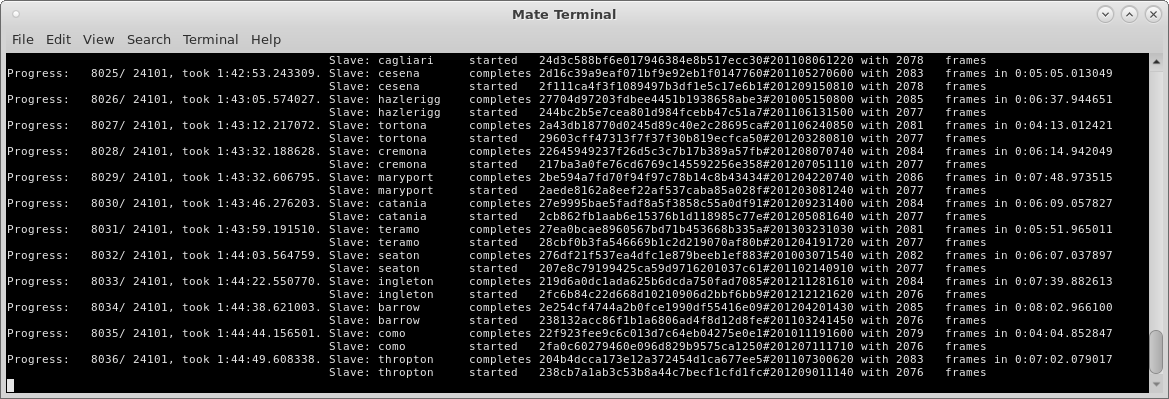
\includegraphics[scale=0.30]{graph/sample_terminal.png}
    \caption{Running the MPI program on MATE terminal}
    \label{fig:mpi}
\end{figure}

\section{CPU Hogging and Memory Thrashing Prevention}

The project uses the public \DIFdelbegin \DIFdel{student lab }\DIFdelend \DIFaddbegin \DIFadd{lab DICE }\DIFaddend machines provided by The University of Edinburgh. 
It is important to make sure the cleaning procedure doesn't affect other \DIFdelbegin \DIFdel{user's work}\DIFdelend \DIFaddbegin \DIFadd{users}\DIFaddend .

A \DIFdelbegin \DIFdel{short bash script combining }\DIFdelend \DIFaddbegin \DIFadd{Python script using Multi-processing pools, spawning a ``}\DIFaddend {\tt \DIFdelbegin \DIFdel{ping}\DIFdelend \DIFaddbegin \DIFadd{ssh MachineName w}\DIFaddend }\DIFdelbegin \DIFdel{and }\DIFdelend \DIFaddbegin \DIFadd{'' bash process for each machine.
With the }\DIFaddend {\tt ssh}\DIFdelbegin \DIFdel{is used to update the }%DIFDELCMD < {\tt %%%
\DIFdel{\$HOSTS}%DIFDELCMD < } %%%
\DIFdel{to a up-to-date }\DIFdelend \DIFaddbegin \DIFadd{'s X11 forwarding enabled, the results printed out at target machine is transferred back to the Python script. 
Then the script checks the length of output obtained from this standard output stream. 
If that machine has no users logged in, the returned string will have an exact length of 2 lines (containing the headers of query). 
This script allows the project to obtain a }\DIFaddend list of available \DIFdelbegin \DIFdel{DICE machines }\DIFdelend \DIFaddbegin \DIFadd{machines within 15 seconds}\DIFaddend .

For the CPU usage, SL7 provides a {\tt NICE} command, allowing the program to have a higher {\tt NI} value which gives lower priority on CPU scheduling. \DIFdelbegin \DIFdel{This allows other students }\DIFdelend \DIFaddbegin \DIFadd{Even if another student logged into the running machine, this allows them }\DIFaddend to work without disruption\DIFdelbegin \DIFdel{by the cleaning}\DIFdelend .

After testing it on the machines, it \DIFdelbegin \DIFdel{is reported }\DIFdelend \DIFaddbegin \DIFadd{was reported anonymously by other students }\DIFaddend that some machines are starting to become unresponsive\DIFaddbegin \DIFadd{, and caused work lost }\DIFaddend after running code on it. \DIFdelbegin %DIFDELCMD < 

%DIFDELCMD < %%%
\DIFdel{Since loading a }\DIFdelend \DIFaddbegin \DIFadd{It is later discovered to be a memory thrashing problem.
Loading a }\DIFaddend video with 10,000 frames and all the library \DIFdelbegin \DIFdel{function used }\DIFdelend \DIFaddbegin \DIFadd{functions }\DIFaddend will take about 3 GB space in physical memory. 
After \DIFdelbegin \DIFdel{unreferencing }\DIFdelend \DIFaddbegin \DIFadd{dereferencing }\DIFaddend every variable and \DIFdelbegin \DIFdel{force }\DIFdelend \DIFaddbegin \DIFadd{forcing }\DIFaddend the garbage collecting mechanism, it still leaves 10\% of the memory in use. This eventually piles up and \DIFdelbegin \DIFdel{thrash }\DIFdelend \DIFaddbegin \DIFadd{thrashes }\DIFaddend the memory. 

A solution is to spawn a sub-process \DIFaddbegin \DIFadd{for each batch of the video cleaning }\DIFaddend and kill it after it's finished\DIFdelbegin \DIFdel{, but this increases }\DIFdelend \DIFaddbegin \DIFadd{. 
Doing so would increase }\DIFaddend the time to reload the \DIFdelbegin \DIFdel{python }\DIFdelend \DIFaddbegin \DIFadd{Python }\DIFaddend libraries, taking about 5 to \DIFdelbegin \DIFdel{60 }\DIFdelend \DIFaddbegin \DIFadd{10 }\DIFaddend seconds per video. 
\DIFaddbegin \DIFadd{The increase in time cost is almost negligible compared to feature extraction cost, so no further optimizations are made. 
}\DIFaddend 

%DIF > Bob: So what did you do?
%DIF > Me:  What?
%DIF > Bob: What?
\DIFaddbegin 

\DIFaddend \section{Error Recovery and Progress Record}

MPI allows a more \DIFaddbegin \DIFadd{portable and }\DIFaddend scalable way of \DIFdelbegin \DIFdel{distribution of task }\DIFdelend \DIFaddbegin \DIFadd{distributing of tasks }\DIFaddend on multiple computational nodes.
However, one of the main \DIFdelbegin \DIFdel{disadvantage }\DIFdelend \DIFaddbegin \DIFadd{disadvantages }\DIFaddend is the error handling\DIFdelbegin \DIFdel{, if }\DIFdelend \DIFaddbegin \DIFadd{. 
If }\DIFaddend one of the \DIFdelbegin \DIFdel{MPI process }\DIFdelend \DIFaddbegin \DIFadd{MPI-process }\DIFaddend crashes, all of the \DIFdelbegin \DIFdel{process }\DIFdelend \DIFaddbegin \DIFadd{processes }\DIFaddend running will be forced to exit.

The project is running on a massive scale, so error handling plays a more and more important role in the processing. 
When an error is caught when processing a video, it immediately sends \DIFaddbegin \DIFadd{the }\DIFaddend master node a {\tt DONE} signal, but with a failure message. The master node will remove the failed slave node and put \DIFdelbegin \DIFdel{it's }\DIFdelend \DIFaddbegin \DIFadd{its }\DIFaddend job back to the start of the work queue, allowing it to be re-scheduled again.

In the case of master crashes and other situations that MPI process is killed, all of the nodes will stop and some progress recording mechanism is needed for resuming progress. After all the output is stored on the disk, another empty file with {\tt .complete} suffix is created. So the \DIFdelbegin \DIFdel{"slave" process }\DIFdelend \DIFaddbegin \DIFadd{``slave'' processes }\DIFaddend could know if a video is finished processing, or killed before it finishes storage. With this file existence check, repeat work after restart is greatly reduced, hence \DIFdelbegin \DIFdel{keeping }\DIFdelend \DIFaddbegin \DIFadd{improving }\DIFaddend the progress.

\DIFaddbegin \DIFadd{Even with these issues addressed, the following event could still cause faults:
}\begin{itemize}
\setlength{\parskip}{0pt}
\item \textbf{\DIFadd{Rebooted machines}}\DIFadd{: Some student tends to restart the lab machines before using them, this causes code to terminated by }{\tt \DIFadd{SIGTERM}} \DIFadd{or }{\tt \DIFadd{SIGKILL}}\DIFadd{.
}\item \textbf{\DIFadd{Unplugged machines}}\DIFadd{: Causes the master node to wait indefinitely for a reply.
}\end{itemize}
\DIFadd{With this limitation, the project could only use the framework during night times.
}

\section{\DIFadd{Time Cost Reduction}} 

\DIFadd{In Yu's thesis\mbox{%DIFAUXCMD
\cite{Yu}}%DIFAUXCMD
, it is estimated the cleaning could take 25,000 hours to complete on a 40-core machine.
This evaluation is based on the runtime of cleaning a video with 961 detections.
Finish processing these videos took approximately 200 seconds, Yu obtain the estimated runtime by multiplying this amount by the total number of the videos (400,000).
Within this 200 seconds, half of the time is used for the SVM feature extraction/transformation, and another half was used for the CNN preprocessing. The final classification took negligible time.
}

\DIFadd{However, this estimate wasn't thorough, since there are 839,000,000 detections and the average length of the video is about 2,000 detections.
The actual runtime would double, having about 1,600,000 hours of runtime on a single core (about 16,000 days on a 4-core machine). 
}

\DIFadd{During the project, about 200 student lab DICE machine was used. 
The number of available DICE machines varies from 50-250 due to heavy experiment period of other students.
This issue potentially cuts the previous runtime to 1/200, but due to the disruption to/from other students, the project runs the cleaning mostly during night time (12 A.M. to 8 A.M.).
}

\DIFadd{With this reduction, the project finishes the different stages in the following time:
}\begin{itemize}
\setlength{\parskip}{0pt}
\item \textbf{\DIFadd{SVM preprocessing}}\DIFadd{: Approximately three weeks, estimated total runtime of about 200 hours. 
}\item \textbf{\DIFadd{CNN preprocessing and classification}}\DIFadd{: Approximately one week, estimated total runtime of 70 hours. 
}\item \textbf{\DIFadd{Other operations}}\DIFadd{: Like training SVM and generating decision vectors, these all took negligible time (less than 1 day). 
}\end{itemize}
\DIFadd{Note that the SVM took longer due to the high memory requirement for the cleaning mentioned in Section \ref{sec:earlyremove}.
}

\DIFadd{Judging from the result cleaning time, the translation stage of the project manages to cut down the runtime to 1/8 of the original speed.
This reduction is mostly the benefit of removing the SQL server, which has brought the project most reduction in runtime. 
It might also be the removal of unnecessary I/O (saving images to disk and loading them again for multiple times) during CNN stage. 
The project benefit mostly from the idle student lab machines, this is equivalent to having 20 40-core machines used in Yu's estimation.
}\DIFaddend \newpage

\chapter{Conclusion}
\label{chap:conclusion}

\section{Project Outcome}

Initially\DIFaddbegin \DIFadd{, }\DIFaddend the project goal \DIFdelbegin \DIFdel{is }\DIFdelend \DIFaddbegin \DIFadd{was }\DIFaddend to further reduce the size of the RDS dataset from 1.6 TB to an acceptable size\DIFdelbegin \DIFdel{, however given }\DIFdelend \DIFaddbegin \DIFadd{. 
Given }\DIFaddend the accuracy obtained from \DIFaddbegin \DIFadd{the }\DIFaddend actual run, doing so would \DIFdelbegin \DIFdel{essentially causing 25\% of the good detections lost in the process}\DIFdelend \DIFaddbegin \DIFadd{not remove enough False Positives}\DIFaddend . Also due to \DIFdelbegin \DIFdel{need of }\DIFdelend \DIFaddbegin \DIFadd{the need for }\DIFaddend maintaining consistency in the {\tt .sql} file and video files, this final \DIFdelbegin \DIFdel{step }\DIFdelend \DIFaddbegin \DIFadd{removal process }\DIFaddend is not used.

Instead, this project produces 2 types of {\tt .npy} file (saved Numpy Arrays). 
One of them is the predicted probability of each class obtained by the 4 major \DIFdelbegin \DIFdel{classifier }\DIFdelend \DIFaddbegin \DIFadd{classifiers }\DIFaddend used, taking about 260 GB disk space. 
Another one is the final binary array of decisions, marking each frame as \DIFaddbegin \DIFadd{a }\DIFaddend good detection or \DIFdelbegin \DIFdel{else, this }\DIFdelend \DIFaddbegin \DIFadd{not. 
This }\DIFaddend is more compact than the other, using about 750 MB disk space.

\DIFdelbegin \DIFdel{Also the }\DIFdelend \DIFaddbegin \DIFadd{The }\DIFaddend by-product of the process may \DIFdelbegin \DIFdel{also }\DIFdelend be useful for \DIFaddbegin \DIFadd{a }\DIFaddend future cleaning attempt on the dataset, this includes:
\begin{itemize}
\DIFaddbegin \setlength{\parskip}{3pt}
\DIFaddend \item A \DIFaddbegin \DIFadd{1 GB folder, contains Numpy dump of final binary decision vector.
}\item \DIFadd{A }\DIFaddend 323 GB folder, contains extracted {\tt .sql} records.
\item A 510 GB folder, contains normalized and PCA transformed first 100 features.
\item About 20,000 marked \DIFaddbegin \DIFadd{frame of }\DIFaddend ground truth dataset, covering the videos both Pugh and Yu \DIFdelbegin \DIFdel{misses during }\DIFdelend \DIFaddbegin \DIFadd{missed during the }\DIFaddend ground truth process.
\item A Python mpi application to distribute the classification work on DICE machines, and a Python script to obtain unused DICE machines.
\item Translated utility functions in Python, some are from Pugh's MATLAB code and some of them are implemented in this project. 
This contains several Jupyter Notebooks \DIFdelbegin \DIFdel{, }\DIFdelend and two Python libraries. 
\DIFdelbegin \DIFdel{Which allows easier visualisation on }\DIFdelend \DIFaddbegin \DIFadd{These allow easier visualisation of }\DIFaddend the dataset, without the need to go through multiple \DIFdelbegin \DIFdel{extraction }\DIFdelend \DIFaddbegin \DIFadd{extractions }\DIFaddend and SQL connection stage in MATLAB. 
\end{itemize}

%DIF < TODO add accuracy when you are done.
\DIFaddbegin \section{\DIFadd{False Negatives in cleaning algorithm}}
\label{sec:falsenegative}
\label{sec:feiffault}
\label{sec:svmfault}
\DIFaddend 

\DIFaddbegin \DIFadd{The cleaning algorithm produces approximately 5-10\% of False Negatives (rejected good fish). 
To reduce the False Negatives, they were scrutinized to see the causing reasons for the fault.
}

\DIFadd{Most of the False Negatives in the cleaning are caused by FEIF used, approximately 2-3\% of the RDS were rejected. 
Fig \ref{fig:feiffail} shows the sample of False Negatives in the validation dataset.
Note that the time-stamp in absent from the area highlighted with red lines.
By looking into the dataset, it is discovered that all the }{\tt \DIFadd{640x480}} \DIFadd{resolution videos recorded at NPP-3 sites after 2011-Aug-05 are missing the time stamp.
}

\begin{figure}[h]
    \centering
    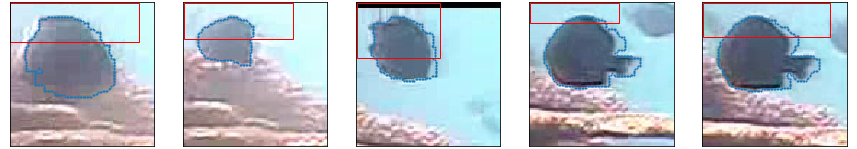
\includegraphics[scale=0.40]{graph/FEIFfail.png}
    \caption{\DIFaddFL{Sample False Negatives (good fish rejected) by FEIF}}
    \label{fig:feiffail}
\end{figure}

\DIFadd{This absence of time stamp was not expected in early stages of the cleaning process, hence it was not included in the settings for FEIF. 
Fig \ref{fig:feiffail2} shows the contours of the False Negative detections.
The darker-red area indicates the time-stamp area for }{\tt \DIFadd{320x240}} \DIFadd{videos used in the species recognition stage of the F4K project, and the light-red area is newly added to this project.
}

\begin{figure}[h]
    \centering
    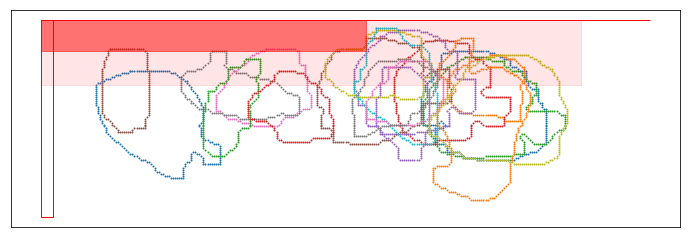
\includegraphics[scale=0.30]{graph/feiffail.png}
    \caption{\DIFaddFL{Contours in the FEIF time-stamp region}}
    \label{fig:feiffail2}
\end{figure}

\DIFadd{The similar problem also happened to the plankton removal criteria in Section \ref{sec:earlyremove}, where a mistake in the time checking code causes some of the videos recorded at 6-7 A.M. to be removed. 
However, this only affects about 0.2\% of the detection.
}

\DIFadd{While the early remove stages fault causes a lot of class 6 False Negative, most of the class 8 False Negative are caused by the SVM used, which is partially considered to be the fault of the classification schema discussed in Section \ref{sec:AmbigCS}.
Where class 8 stands for good fish with bad contour, this covers detections from slightly erratic contour to completely useless contour.
Fig \ref{fig:SVMfail} shows the sample of such fault, these contour fault caused by background extraction of previous species recognition of F4K project.
Fishes with colours similar to the background or stripes usually have broken or segmented contours.
}

\begin{figure}[h]
    \centering
    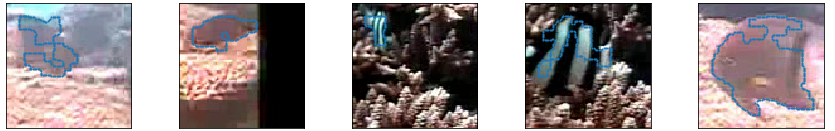
\includegraphics[scale=0.40]{graph/SVMfail.png}
    \caption{\DIFaddFL{Sample False Negatives (good fish rejected) by SVM}}
    \label{fig:SVMfail}
\end{figure}

\DIFaddend \section{Future Work}
\label{sec:future}

This project successfully \DIFdelbegin \DIFdel{applies }\DIFdelend \DIFaddbegin \DIFadd{applied }\DIFaddend the cleaning algorithms designed by Pugh\cite{Pugh}\DIFdelbegin \DIFdel{, however }\DIFdelend \DIFaddbegin \DIFadd{. 
Unfortunately, }\DIFaddend it did not achieve the same level of accuracy as Pugh's thesis described.
In order to increase the accuracy of the classifiers, \DIFdelbegin \DIFdel{following improvements will }\DIFdelend \DIFaddbegin \DIFadd{not only we need to fix the aforementioned faults in Section \ref{sec:falsenegative}, other improvements will also }\DIFaddend be needed.

\subsection{More Annotation}

As stated in Section \ref{sec:gt}, the current Ground Truth Dataset is heavily biased, which completely misses out the detections at some \DIFdelbegin \DIFdel{site }\DIFdelend \DIFaddbegin \DIFadd{sites }\DIFaddend of filming. 
Even after adding 20,000 detections across every site, the dataset still \DIFdelbegin \DIFdel{have }\DIFdelend \DIFaddbegin \DIFadd{has }\DIFaddend incomplete coverage on the RDS. 

Pugh also mentioned about this problem in his thesis, where more human annotator might be needed for the project.
With the limitation of the current classification schema, the ground truth process is irritating and tedious due to the ambiguity mentioned in Section \ref{sec:AmbigCS}.

An alternative \DIFdelbegin \DIFdel{maybe }\DIFdelend \DIFaddbegin \DIFadd{may be }\DIFaddend using an online survey for ground truth\DIFdelbegin \DIFdel{, however it }\DIFdelend \DIFaddbegin \DIFadd{. 
But the survey }\DIFaddend is not fully implemented at this stage of the project. 
\DIFaddbegin \DIFadd{Fig \ref{fig:gto} shows the web interface for the survey.
A user is shown a detection in a track, and they could use the provided options to send their decision to the database server used.
}\DIFaddend 

\begin{figure}[!h]
    \centering
    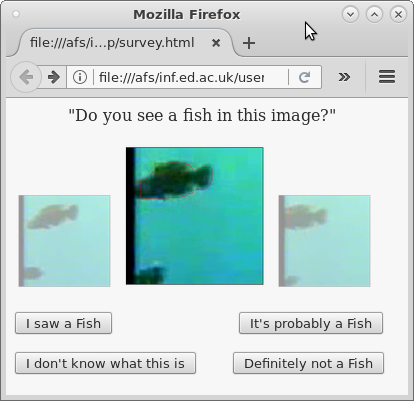
\includegraphics[scale=0.38]{graph/query.png}
    \caption{A prototype online ground truth interface}
    \label{fig:gto}
\end{figure}

\subsection{Training New CNNs}

Due to the image extraction fault in the training stage of the CNN, \DIFdelbegin \DIFdel{a }\DIFdelend \DIFaddbegin \DIFadd{an }\DIFaddend over-fitted version of CNN is used in this project. 
In order to achieve expected accuracy in Pugh's thesis\cite{Pugh}, \DIFdelbegin \DIFdel{re-train }\DIFdelend \DIFaddbegin \DIFadd{re-training }\DIFaddend of the network will be needed.

The accuracy obtained by the training dataset on CNN\_WC has shown promising accuracy even with \DIFdelbegin \DIFdel{completely wrong color }\DIFdelend \DIFaddbegin \DIFadd{a completely wrong colour }\DIFaddend space. Combining with Pugh's result obtained in \DIFaddbegin \DIFadd{the }\DIFaddend experiment stage, and the difference in performance on Training/Validation dataset obtained in this project, it's almost certain \DIFaddbegin \DIFadd{that }\DIFaddend a well-trained CNN would obtain at least 70\% accuracy on the cleaning task. 

\section{Final Words}
%DIF < TODO shuai-guo

%DIF <  use the following and \cite{} as above if you use BibTeX
%DIF <  otherwise generate bibtem entries
\DIFaddbegin \DIFadd{The project manages to finish the algorithm originally designed by Pugh. However, the expected level of accuracy was not achieved.
In hindsight, the developing process was not careful enough, which is mainly reflected in the FEIF behaviour of the project. 
While setting parameters, only reduction rate is considered. 
Details like False Negative Rate was ignored and have led to most of the detection lost.
}

\DIFadd{Also, the project has trusted the previous result blindly at early stages of the cleaning, which has led to the late discovery of the CNN fault.
The validation dataset is marked only after the translation of the algorithms.
}

\DIFadd{With the big data nature of this task, many issues only arise when the project started running the cleaning on the distributed scale.
These issues could be avoided if enough test was created at the start of the project.
}

\DIFadd{For example, MATLAB's ParPool uses a local lock file to keep track of the parallel tasks. 
Combined with the shared file system used, lots of MATLAB segmentation fault crashes have been caused because of this. 
Due to the ambiguity of the error messages, this problem is only addressed months after first discovery.
}

\DIFadd{Another example would be the }{\tt \DIFadd{.sql}} \DIFadd{preprocessing mentioned in Section \ref{sec:sqld}.
The project misses one of the special characters in the blob syntax used, which has caused 30\% of the contour data appears to be missing after extraction.
This fault also causes the project to re-run the SVM extraction stage and 2 week's work were lost because of it.
}

\DIFadd{Future work on the project is needed to fix the existing fault. 
Exploration of other machine learning techniques is also needed in order to achieve higher accuracy on the classification. 
}





\DIFaddend \bibliographystyle{unsrt}
\bibliography{dissertation}
\DIFaddbegin 


\begin{appendices}

\chapter{\DIFadd{Master/Slave Framework Pseudo-Code}}
\label{apped:msf}

\DIFadd{With this framework design, if we want to process any stage of the pipeline classifier, we only need to overwrite the dummy }\underline{\textbf{\DIFadd{DoWork}}\DIFadd{(VideoID)}} \DIFadd{function of slave code.
}

\DIFadd{If the framework is used in work other than processing the videos, (e.g. finding SVM parameters), the  }\underline{\textbf{\DIFadd{VideoIDList}}} \DIFadd{can be changed to adapt the new tasks.
}

\begin{center}
\vspace{10pt}
\textbf{\DIFadd{Code removed for generating diff.}}
\vspace{10pt}
\end{center}

\chapter{\DIFadd{Sample of Lengthy Videos}}
\label{append:samplelong}

\DIFadd{In Section \ref{sec:earlyremove}, a classification method based on file-name is proposed.
If a video has over 30,000 frames and is filmed at a specific time and location, every frame of the video will be marked as non-fish. 
As each video of RDS originates from a 10-minute video, having such amount of detection essentially means there are over 50 fish captured per second of original FDS.
}

\DIFadd{For the most of the cases, such videos are full of compression errors, plankton, or having background extraction fault caused by moving vegetation. These cases are shown in Fig \ref{fig:sample_night}, Fig \ref{fig:sample_corrupt}, and Fig \ref{fig:sample_vegetation}.
}

\DIFadd{By manually looking through the samples from the longest videos, a limit of 30,000 is set due to the need of keeping good detections such as those in Fig \ref{fig:sample_fish}. This ensures the good fish lost will be less than 1\% of the bad detections this method removes.
}

\begin{figure}
\centering
    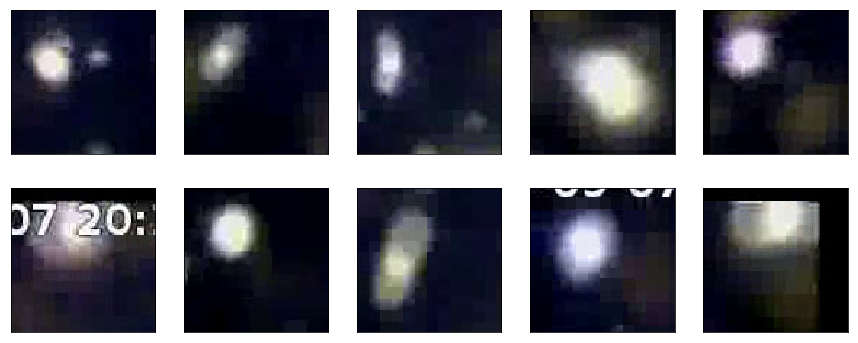
\includegraphics[scale=0.46]{graph/sample_night.png}
    \caption{\DIFaddFL{Sample frames from a video filmed at night.}}
    \label{fig:sample_night}
\end{figure}

\begin{figure}
\centering
    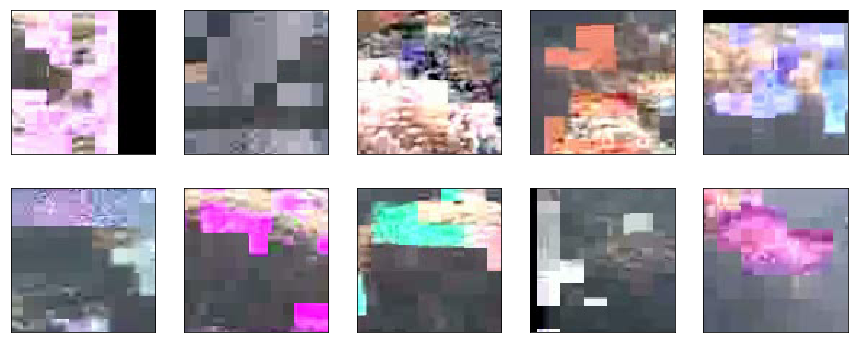
\includegraphics[scale=0.46]{graph/sample_corrupt.png}
    \caption{\DIFaddFL{Sample frames from a corrupted video.}}
    \label{fig:sample_corrupt}
\end{figure}

\begin{figure}
\centering
    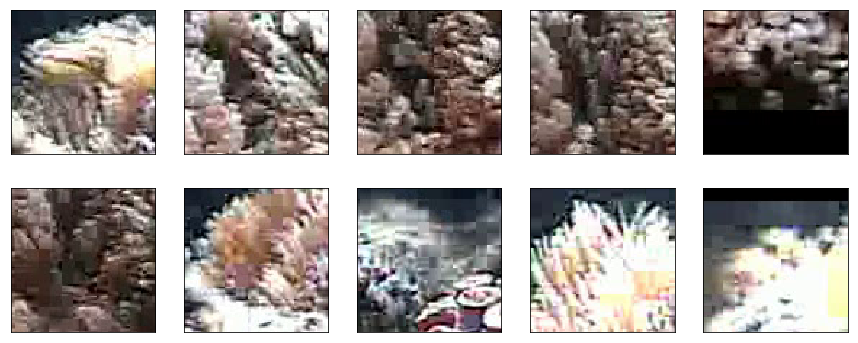
\includegraphics[scale=0.46]{graph/sample_vegetation.png}
    \caption{\DIFaddFL{Sample frames from a video with dynamic background.}}
    \label{fig:sample_vegetation}
\end{figure}
\begin{figure}
\centering
    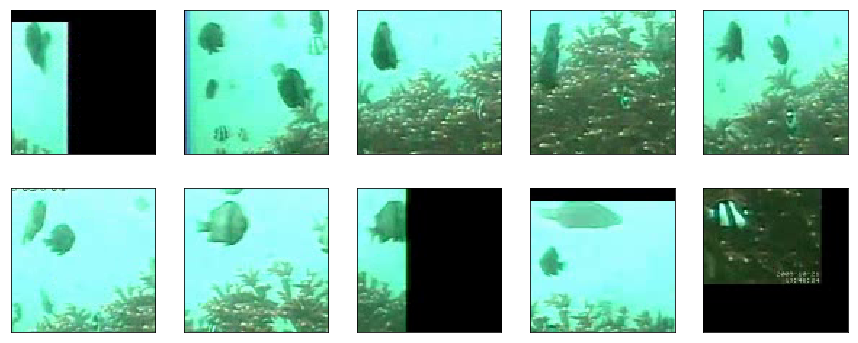
\includegraphics[scale=0.46]{graph/sample_fish.png}
    \caption{\DIFaddFL{Sample frames from a video with abnormal amount of fish.}}
    \label{fig:sample_fish}
\end{figure}

\end{appendices}
\DIFaddend 

\end{document}
